%\documentclass[compress]{beamer}
\documentclass[8pt]{beamer}

%-----------------------------------------------------------
% PACKAGES

%\usepackage[latin1]{inputenc}
\mode<presentation>

%\usepackage[T1]{fontenc}  
\usetheme{Warsaw}

\usepackage{graphicx}
%\usepackage[section]{placeins} % force � mettre l'image o� on veut
%\usepackage{float} %utiliser H pour forcer � mettre l'image o� on veut
\usepackage{lscape} %utilisation du mode paysage
%\usepackage{pslatex}
\usepackage{url}
%\usepackage{subfigure}
\usepackage{caption}
\usepackage{subcaption}

\usepackage{graphicx}
\usepackage{tabls}
\usepackage{afterpage}

%\usepackage[]{media9}
\usepackage{multimedia}

\usepackage{amsthm}
\usepackage{amssymb}
\usepackage{amsmath}
\usepackage{amsfonts}
\usepackage{amstext}
\usepackage{amsbsy}
\usepackage{mathbbol} 


\usepackage{epsfig}
%\usepackage{epsfig}
%\usepackage{cites}
\usepackage{epsf}
\usepackage{array}
\usepackage{color}

%-----------------------------------------------------------
% NEW  DEFINITIONS
%
%=================================================================================================
% new commands
% +++++++++++++++++++++++++++++++++++++++++++++++++++++++++++++++++++++++++++++++++++++++++++++++++
\newcommand{\nc}{\newcommand}
%
% Ways of grouping things
%
\newcommand{\bracket}[1]{\left[ #1 \right]}
\newcommand{\bracet}[1]{\left\{ #1 \right\}}
\newcommand{\fn}[1]{\left( #1 \right)}
\newcommand{\ave}[1]{\left\langle #1 \right\rangle}
%
% Derivative forms
% 
\newcommand{\dx}[1]{\,d#1}
\newcommand{\dxdy}[2]{\frac{\partial #1}{\partial #2}}
\newcommand{\dxdt}[1]{\frac{\partial #1}{\partial t}}
\newcommand{\dxdz}[1]{\frac{\partial #1}{\partial z}}
\newcommand{\dfdt}[1]{\frac{\partial}{\partial t} \fn{#1}}
\newcommand{\dfdz}[1]{\frac{\partial}{\partial z} \fn{#1}}
\newcommand{\ddt}[1]{\frac{\partial}{\partial t} #1}
\newcommand{\ddz}[1]{\frac{\partial}{\partial z} #1}
\newcommand{\dd}[2]{\frac{\partial}{\partial #1} #2}
\newcommand{\ddx}[1]{\frac{\partial}{\partial x} #1}
\newcommand{\ddy}[1]{\frac{\partial}{\partial y} #1}
%
% Vector forms
%
%\renewcommand{\vec}[1]{\ensuremath{\stackrel{\rightarrow}{#1}}}
%\renewcommand{\div}{\ensuremath{\vec{\nabla} \cdot}}
%\newcommand{\grad}{\ensuremath{\vec{\nabla}}}

\renewcommand{\div}{\vec{\nabla}\! \cdot \!}
\newcommand{\grad}{\vec{\nabla}}
\newcommand{\oa}[1]{\fn{\frac{1}{3}\hat{\Omega}\!\cdot\!\overrightarrow{A_{#1}}}}

%
% Equation beginnings and endings
%
\newcommand{\bea}{\begin{eqnarray}}
\newcommand{\eea}{\end{eqnarray}}
\newcommand{\be}{\begin{equation}}
\newcommand{\ee}{\end{equation}}
\newcommand{\beas}{\begin{eqnarray*}}
\newcommand{\eeas}{\end{eqnarray*}}
\newcommand{\bdm}{\begin{displaymath}}
\newcommand{\edm}{\end{displaymath}}
%
% Equation punctuation
% 
\newcommand{\pec}{\hspace{0.25in},}
\newcommand{\pep}{\hspace{0.25in}.}
\newcommand{\pev}{\hspace{0.25in}}
%
% Equation labels and references, figure references, table references
% 
\newcommand{\LEQ}[1]{\label{eq:#1}}
\newcommand{\EQ}[1]{Eq.~(\ref{eq:#1})}
\newcommand{\EQS}[1]{Eqs.~(\ref{eq:#1})}
\newcommand{\REQ}[1]{\ref{eq:#1}}
\newcommand{\LFI}[1]{\label{fi:#1}}
\newcommand{\FI}[1]{Fig.~\ref{fi:#1}}
\newcommand{\RFI}[1]{\ref{fi:#1}}
\newcommand{\LTA}[1]{\label{ta:#1}}
\newcommand{\TA}[1]{Table~\ref{ta:#1}}
\newcommand{\RTA}[1]{\ref{ta:#1}}

%
% List beginnings and endings
% 
\newcommand{\bl}{\bss\begin{itemize}}
\newcommand{\el}{\vspace{-.5\baselineskip}\end{itemize}\ess}
\newcommand{\benu}{\bss\begin{enumerate}}
\newcommand{\eenu}{\vspace{-.5\baselineskip}\end{enumerate}\ess}
%
% Figure and table beginnings and endings
% 
\newcommand{\bfg}{\begin{figure}}
\newcommand{\efg}{\end{figure}}
\newcommand{\bt}{\begin{table}}
\newcommand{\et}{\end{table}}
%
% Tabular and center beginnings and endings
% 
\newcommand{\bc}{\begin{center}}
\newcommand{\ec}{\end{center}}
\newcommand{\btb}{\begin{center}\begin{tabular}}
\newcommand{\etb}{\end{tabular}\end{center}}
%
% Single space command
% 
%\newcommand{\bss}{\begin{singlespace}}
%\newcommand{\ess}{\end{singlespace}}
\newcommand{\bss}{\singlespacing}
\newcommand{\ess}{\doublespacing}
%
%---New environment "arbspace". (modeled after singlespace environment
%                                in Doublespace.sty)
%   The baselinestretch only takes effect at a size change, so do one.
% 
\def\arbspace#1{\def\baselinestretch{#1}\@normalsize}
\def\endarbspace{}
\newcommand{\bas}{\begin{arbspace}}
\newcommand{\eas}{\end{arbspace}}
%
% An explanation for a function
%
\newcommand{\explain}[1]{\mbox{\hspace{2em} #1}}
%
% Quick commands for symbols
%  
\newcommand{\half}{\frac{1}{2}}
\newcommand{\third}{\frac{1}{3}}
\newcommand{\twothird}{\frac{2}{3}}
\newcommand{\fourth}{\frac{1}{4}}
\newcommand{\mdot}{\dot{m}}
\newcommand{\ten}[1]{\times 10^{#1}\,}
\newcommand{\cL}{{\cal L}}
\newcommand{\cD}{{\cal D}}
\newcommand{\cF}{{\cal F}}
\newcommand{\cE}{{\cal E}}
\renewcommand{\Re}{\mbox{Re}}
\newcommand{\Ma}{\mbox{Ma}}
%
% Inclusion of Graphics Data
%
%\input{psfig}
%\psfiginit
%
% More Quick Commands
% 
\newcommand{\bi}{\begin{itemize}}
\newcommand{\ei}{\end{itemize}}
\newcommand{\ben}{\begin{enumerate}}
\newcommand{\een}{\end{enumerate}}
\newcommand{\dxi}{\Delta x_i}
\newcommand{\dyj}{\Delta y_j}
\newcommand{\ts}[1]{\textstyle #1}


\newcommand{\bu}{\boldsymbol{u}}
\newcommand{\ber}{\boldsymbol{e}}
\newcommand{\br}{\boldsymbol{r}} 
\newcommand{\bo}{\boldsymbol{\Omega}}

\newcommand{\bn}{\boldsymbol{\nabla}}

% DGFEM commands
\newcommand{\jmp}[1]{[\![#1]\!]}                     % jump
\newcommand{\mvl}[1]{\{\!\!\{#1\}\!\!\}}             % mean value


\newcommand{\boxedeqn}[1]{%
  \[\fbox{%
      \addtolength{\linewidth}{-2\fboxsep}%
      \addtolength{\linewidth}{-2\fboxrule}%
      \begin{minipage}{\linewidth}%
      \begin{equation}#1\end{equation}%
      \end{minipage}%
    }\]%
}
\newcommand{\mboxed}[1]{\boxed{\phantom{#1}}}
\newcommand{\ud}{\,\mathrm{d}}

% keff
\newcommand{\keff}{\ensuremath{k_{\textit{eff}}}\xspace}

% margin par
\newcommand{\mt}[1]{\marginpar{ {\footnotesize #1} }}

% shortcut for aposterio in italics
\newcommand{\apost}{\textit{a posteriori\xspace}}
\newcommand{\Apost}{\textit{A posteriori}\xspace}

% shortcut for multi-group
\newcommand{\mg}{multigroup\xspace}
\newcommand{\Mg}{Multigroup\xspace}
\newcommand{\ho}{higher-order\xspace}
\newcommand{\Ho}{Higher-order\xspace}
\newcommand{\HO}{Higher-Order\xspace}
\newcommand{\HObig}{HIGHER-ORDER\xspace}
\newcommand{\Mgbig}{MULTIGROUP\xspace}

% shortcut for domain notation
\newcommand{\D}{\mathcal{D}}

% shortcut for xuthus
\newcommand{\psc}[1]{{\sc {#1}}}
\newcommand{\xuthus}{\psc{xuthus}\xspace}

% vector shortcuts
\newcommand{\vo}{\vec{\Omega}}
\newcommand{\vr}{\vec{r}}
\newcommand{\vn}{\vec{n}}
\newcommand{\vnk}{\vec{\mathbf{n}}}

% extra space
\newcommand{\qq}{\quad\quad}

% sign function
\DeclareMathOperator{\sgn}{sgn}


\newcommand{\ensuretext}[1]{\ensuremath{\text{#1}}}

% common reference commands
\newcommand{\eqt}[1]{Eq.~(\ref{#1})}                     % equation
\newcommand{\fig}[1]{Fig.~\ref{#1}}                      % figure
\newcommand{\tbl}[1]{Table~\ref{#1}}                     % table



\newcommand{\rhs}{right-hand-side\xspace}
\newcommand{\clearemptydoublepage}{\newpage{\pagestyle{empty}\cleardoublepage}}




\newcommand{\bs}[1]{\mathbf{#1}}
\renewcommand{\bs}[1]{\vec{#1}}
%\newcommand{\dd}{\mathrm{d}}
\newcommand{\norm}{\textrm{norm}}
\renewcommand{\Re}{\textrm{Re}}
\newcommand{\Pe}{\textrm{P\'e}}
\renewcommand{\Pr}{\textrm{Pr}}

\newcommand{\resi}{R_e}
%\newcommand{\resinew}{\tilde{D}_e}
\newcommand{\resinew}{\widetilde{\resi}}
\newcommand{\matder}[1]{\frac{\textrm{D} #1}{\textrm{D} t}}

\newcommand{\divv}[1]{\vec{\nabla}^{#1}\! \cdot \!}
\newcommand{\gradd}[1]{\vec{\nabla}^{#1}}

\newcommand{\tcr}[1]{\textcolor{red}{#1}}
\newcommand{\tcb}[1]{\textcolor{blue}{#1}}
\newcommand{\tcm}[1]{\textcolor{magenta}{#1}}

%=================================================================================================

%============================================================

%style et couleur
%\usetheme{Frankfurt}
\date{09/30/2014}

%\addtobeamertemplate{footline}{\hfill\insertframenumber/\inserttotalframenumber\hspace{2em}\null}

\setbeamertemplate{footline}{
\leavevmode%
%\hbox{\hspace*{-0.06cm}
\begin{beamercolorbox}[wd=.5\paperwidth,ht=3.25ex,dp=1ex,center]{author in head/foot}%
	\usebeamerfont{author in head/foot}\insertshortauthor%~~(\insertshortinstitute)
\end{beamercolorbox}%
\begin{beamercolorbox}[wd=.25\paperwidth,ht=3.25ex,dp=1ex,center]{section in head/foot}%
	\usebeamerfont{section in head/foot} PHYSOR-2014 % \insertshorttitle
\end{beamercolorbox}%
\begin{beamercolorbox}[wd=.25\paperwidth,ht=3.25ex,dp=1ex,left]{section in head/foot}%
	\usebeamerfont{section in head/foot}\insertshortdate{}\hspace*{2em}
	\insertframenumber{} / \inserttotalframenumber %\hspace*{2ex}
\end{beamercolorbox}}%
%\vskip0pt%
%}

\beamertemplatetransparentcovered

\urldef{\ragusa}\url{jean.ragusa@tamu.edu}
\urldef{\delchini}\url{delcmo@tamu.edu}
\urldef{\berry}\url{ray.berry@inl.gov}

\title{Extension of the entropy viscosity method to the low-Mach regime for the multi-dimensional Euler equations}

\author{Marc O. Delchini$^\star$, Jean C. Ragusa$^\star$, Ray Berry$^\ddagger$}
\institute{
$^\star$   Texas A\&M University, College Station, TX, USA\\
$^\dagger$ Idaho National Laboratory, Idaho Falls, ID, USA}

%%%%%%%%%%%%%%%%%%%%%%%%%%%%%%%%%%%%%%%%%%%%%%%%%%%%%%%%%%%%%%%%%%%%

\begin{document}

\begin{frame}
\titlepage
\small{email:  {\delchini}, {\ragusa}, {\berry} }

\end{frame}

\begin{frame}
	\frametitle{Outline}
	\tableofcontents 
\end{frame}

%%%%%%%%%%%%%%%%%%%%%%%%%%%%%%%%%%%%%%%%%%%%%%%%%%%%%%%%%%%%%%%%%%%%
%%%%%%%%%%%%%%%%%%%%%%%%%%%%%%%%%%%%%%%%%%%%%%%%%%%%%%%%%%%%%%%%%%%%
\section{Background and Motivation}
%%%%%%%%%%%%%%%%%%%%%%%%%%%%%%%%%%%%%%%%%%%%%%%%%%%%%%%%%%%%%%%%%%%%
%%%%%%%%%%%%%%%%%%%%%%%%%%%%%%%%%%%%%%%%%%%%%%%%%%%%%%%%%%%%%%%%%%%%

%%%%%%%%%%%%%%%%%%%%%%%%%%%%%%%%%%%%%%%%%%%%%%%%%%%%%%%%%%%%%%%%%%%%
\subsection{Relap-7: a Next-generation nuclear reactor safety code}
%%%%%%%%%%%%%%%%%%%%%%%%%%%%%%%%%%%%%%%%%%%%%%%%%%%%%%%%%%%%%%%%%%%%



%%%%%%%%%%%%%%%%%%%%%%%%%%%%%%%%%%%%%%%%%%%%%%%%%%%%%%%%%%%%%%%%%%%%
\begin{frame} 
\frametitle{The RELAP (Reactor Excursion and Leak Analysis Program) family of codes}

Current industry standard: RELAP-5 (mod 3.2)\\
\begin{itemize}
\item 6-equation two-phase flow model with time- and volume-averaged equations. The 6-eq model is ill-posed (non hyperbolic) and needs artificial viscosity and surface tension to be well-posed.
\item Semi-implicit in time with staggered spatial grids (momentum grid half-shifted from the mass/energy grid)
\item Original model developed in the mid 1970s-early 1980s with continued enhancements since then.
\end{itemize}

\begin{block}{\tcm{Relap-7}: next-generation reactor safety code}
\begin{itemize}
\item \tcr{Goal}: To develop the next-generation reactor safety code by leveraging advances in numerical methods and computer hardware
\item \tcr{Means}: Use \tcm{MOOSE} (Multiphysics Object-Oriented Simulation Environment) to solve the multiphysics problem
\begin{itemize}
\item Fully implicitly in time (BDF-2 time integration)
\item Jacobian-free Newton Krylov for nonlinear solves
\item Leverage from existing libraries: Finite Element Method (\tcm{libmesh}), linear/nonlinear solve libraries (\tcm{PETSc, Hypre})
\end{itemize}
\end{itemize}
\end{block}

\end{frame}

\begin{frame} 
\frametitle{MOOSE: Multiphysics Object-Oriented Simulation Environment}

\begin{block}{MOOSE}
\begin{itemize}
\item Open-source since March 2014: {\tt www.mooseframework.org}, 
\item R\&D Mag 100-award winners {\tt http://www.rdmag.com/award-winners/2014/07/2014-r-d-100-award-winners}
%\item \texttt{www.inl.gov/research/moose-applications/}
\end{itemize}

Many multiphysics \tcm{MOOSE-applications} already built using MOOSE:
\begin{enumerate}
\item BISON (thermo�mechanical fuel performance)
\item MARMOT (mesa-scale modeling of microscopic fuel changes during irradiation) 
\item RattleS$_\text{N}$ake ($S_N$ neutron transport)
\item RELAP-7 
\item \ldots
\end{enumerate}
\end{block}

\begin{block}{Other Relap-7 talk}
\hspace{0.5cm} $\bullet$ 
\tcb{Tuesday Nov. 11, 10:10AM:} {\it Status Update on RELAP-7: A Next Generation Reactor System
Analysis Code},
Richard Martineau, Hongbin Zhang, Haihua Zhao,
Ling Zou (INL) \\
\hspace{0.5cm} $\bullet$ 
\tcb{Tuesday Nov. 11, 2:40AM:} {\it Methodology for the Incorporation of Passive Component Aging
Modeling into the RAVEN/RELAP-7Environment}, A. Guler, D. Mandelli, A. Alfonsi, J.  Cogliati, C. Rabiti, T. Aldemir
\end{block}


\end{frame}
%%%%%%%%%%%%%%%%%%%%%%%%%%%%%%%%%%%%%%%%%%%%%%%%%%%%%%%%%%%%%%%%%%%%





%%%%%%%%%%%%%%%%%%%%%%%%%%%%%%%%%%%%%%%%%%%%%%%%%%%%%%%%%%%%%%%%%%%%
\subsection{Density-based (compressible) Solvers for Low-Mach Flow Problems}
%%%%%%%%%%%%%%%%%%%%%%%%%%%%%%%%%%%%%%%%%%%%%%%%%%%%%%%%%%%%%%%%%%%%


%%%%%%%%%%%%%%%%%%%%%%%%%%%%%%%%%%%%%%%%%%%%%%%%%%%%%%%%%%%%%%%%%%%%
\begin{frame} 
\frametitle{All-speed fluid flow solver}

\begin{block}{Goal}
To use \tcm{compressible} fluid equations for \tcm{all Mach} numbers\\
To solve them using \textcolor{red}{{\it continuous} FEM} using MOOSE 
\end{block}

\begin{block}{All-speed fluid flow solver}
Low-Mach: huge disparity in speeds (pressure waves move much faster)\\
\hspace{0.5cm} $\bullet$ Severely CFL-constrained if using explicit time-stepping\\
\hspace{0.5cm} $\bullet$ Best to use \tcr{implicit} time stepping \\
\hspace{0.5cm} $\bullet$ Nonlinear system of equations \\%(preconditioner: pressure-correction ICE, for example)\\
\hspace{0.5cm} $\bullet$ Fits the JFNK formalism in MOOSE where all physic components are tightly coupled \\
\end{block}

\begin{block}{Regularization technique for discretization of fluid flow}
We will employ novel artificial viscosity schemes based on the entropy production residual
\small{ (Guermond et al., {\it Entropy viscosity method for nonlinear  conservation laws}, J. of Comput. Phys. (2011).}\\
\medskip
The \tcm{entropy viscosity method} is \tcr{discretization-independent} and was significantly tested in the supersonic regime
(including using \tcr{continuous FEM}).
\end{block}



\end{frame}
%%%%%%%%%%%%%%%%%%%%%%%%%%%%%%%%%%%%%%%%%%%%%%%%%%%%%%%%%%%%%%%%%%%%


%%%%%%%%%%%%%%%%%%%%%%%%%%%%%%%%%%%%%%%%%%%%%%%%%%%%%%%%%%%%%%%%%%%%
%%%%%%%%%%%%%%%%%%%%%%%%%%%%%%%%%%%%%%%%%%%%%%%%%%%%%%%%%%%%%%%%%%%%
\section{A Brief Review of the Entropy Viscosity Method for Conservation Laws}
%%%%%%%%%%%%%%%%%%%%%%%%%%%%%%%%%%%%%%%%%%%%%%%%%%%%%%%%%%%%%%%%%%%%
%%%%%%%%%%%%%%%%%%%%%%%%%%%%%%%%%%%%%%%%%%%%%%%%%%%%%%%%%%%%%%%%%%%%

%%%%%%%%%%%%%%%%%%%%%%%%%%%%%%%%%%%%%%%%%%%%%%%%%%%%%%%%%%%%%%%%%%%%
\subsection{Basic Idea}
%%%%%%%%%%%%%%%%%%%%%%%%%%%%%%%%%%%%%%%%%%%%%%%%%%%%%%%%%%%%%%%%%%%%


%%%%%%%%%%%%%%%%%%%%%%%%%%%%%%%%%%%%%%%%%%%%%%%%%%%%%%%%%%%%%%%%%%%%
\begin{frame} 
\frametitle{Quick overview of the entropy-based artificial viscosity formalism}

General scalar conservation law: $\partial_t u + \div \vec{f}(u) = 0$.

\begin{enumerate}
\item Determine an entropy pair ($s(u),\, \vec{\Psi}(u)$) for the PDE under consideration
\item Compute the entropy residual $R_e:=\partial_t s(u_h) + \div \Psi(u_h)$, in each cell $K$, at each quadrature point $x_q$
\item Compute the speed associated with this residual
\be
v_e := h \frac{|R_e(x_q)|_K}{|s-\overline{s}|_\infty}
\ee
%The denominator is used to normalize the residual
%. It is the deviation of $E(u)$ from the domain average $\overline{E}$.
\item Define the dynamic viscosity (m$^2$/s) as
\be
\mu := h \min \Big( \frac{1}{2} |\vec{f}'(u)|, \, v_e \Big)
\ee
\item Plug in the standard Galerkin weak form as a \tcm{viscous regularization} %(\tcm{it is really a straightforward technique})
\be
\int_V \big( \partial_t u_h + \div \vec{f}(u_h) \big) b \, dx + \tcm{\sum_K \int_K \mu_K \grad u_h \grad b \, dx} = 0 \quad \forall b
\ee
\end{enumerate}


\end{frame}
%%%%%%%%%%%%%%%%%%%%%%%%%%%%%%%%%%%%%%%%%%%%%%%%%%%%%%%%%%%%%%%%%%%%

%%%%%%%%%%%%%%%%%%%%%%%%%%%%%%%%%%%%%%%%%%%%%%%%%%%%%%%%%%%%%%%%%%%%
%\begin{frame} 
%\frametitle{Example: Burgers equation}
%\begin{figure}
%	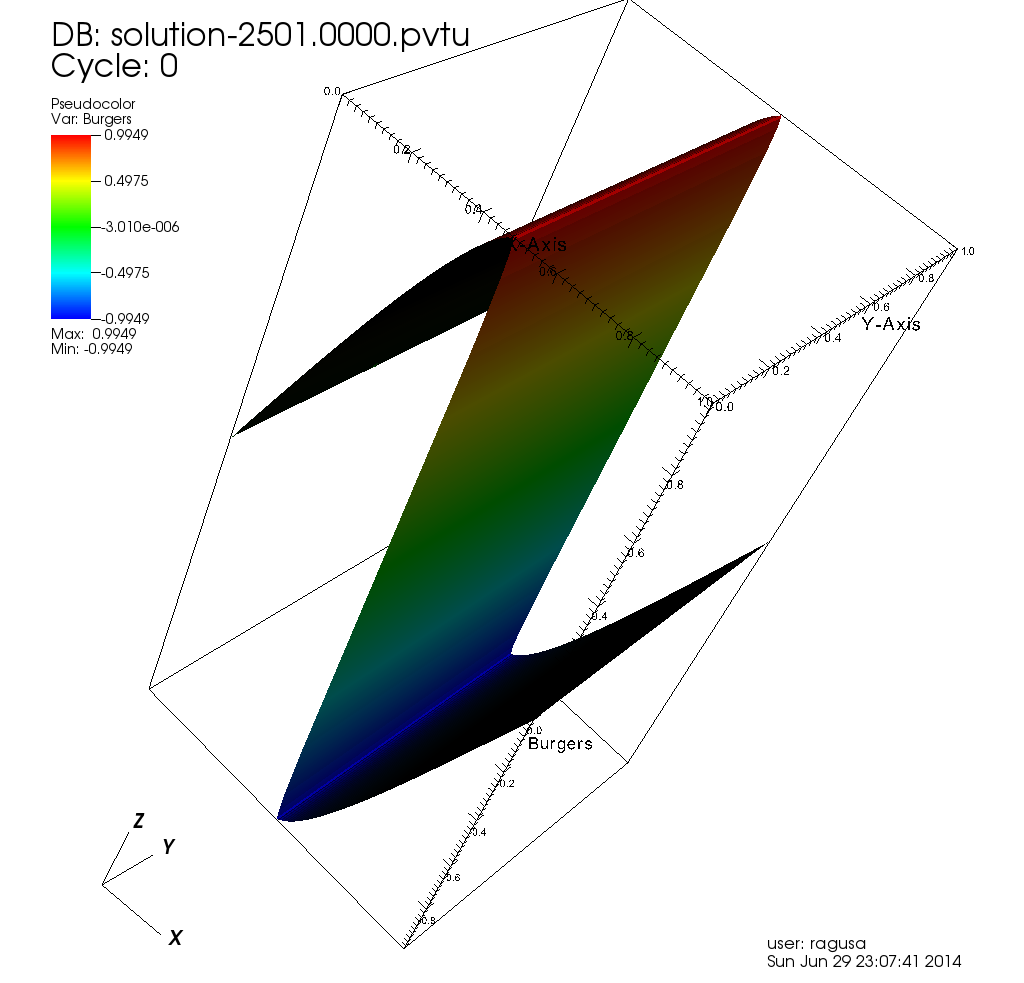
\includegraphics[height=7cm, keepaspectratio=true]{figs/burgers0000.png}
%\end{figure}
%\end{frame}
%
%\begin{frame} 
%\begin{figure}
%	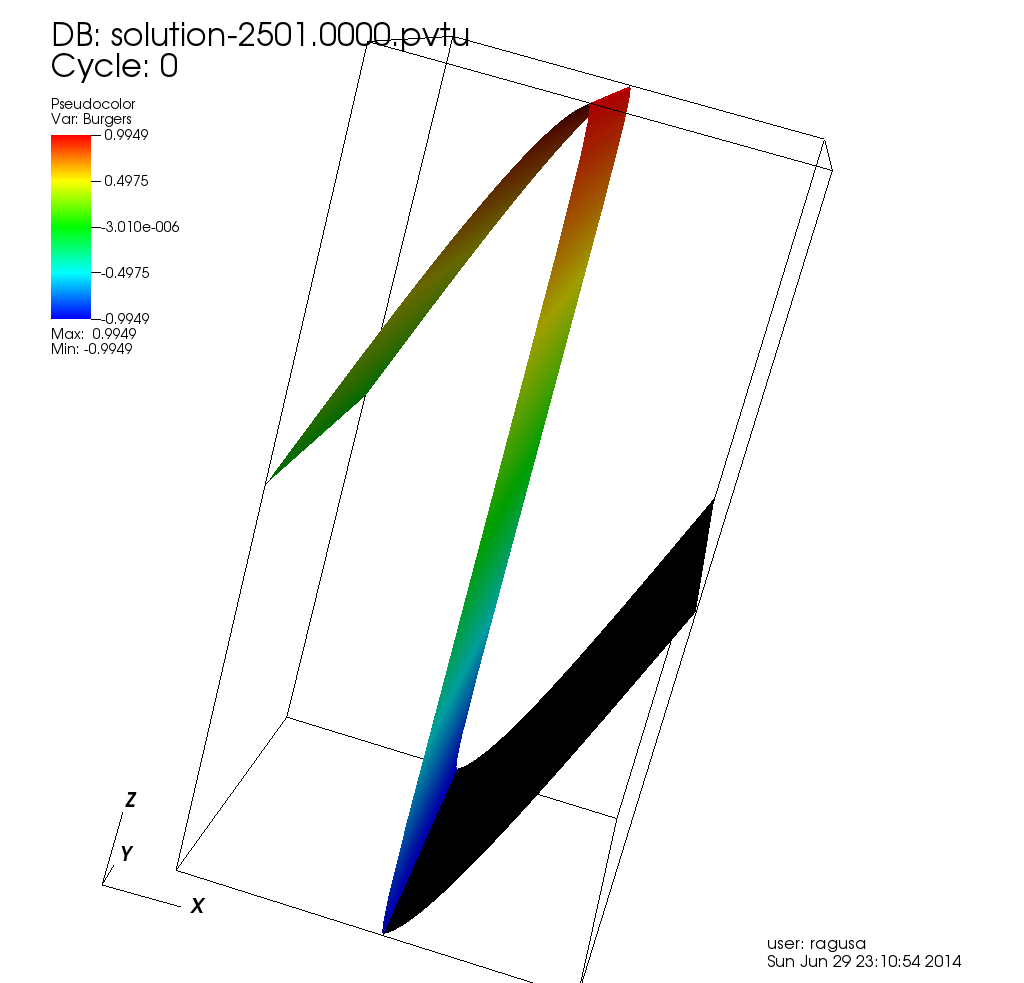
\includegraphics[height=7cm, keepaspectratio=true]{figs/burgers20000.png}
%\end{figure}
%\end{frame}

\begin{frame}
\frametitle{Example: Burgers equation}
\begin{figure}
        \centering
        \begin{subfigure}[b]{0.37\textwidth}
                \centering
                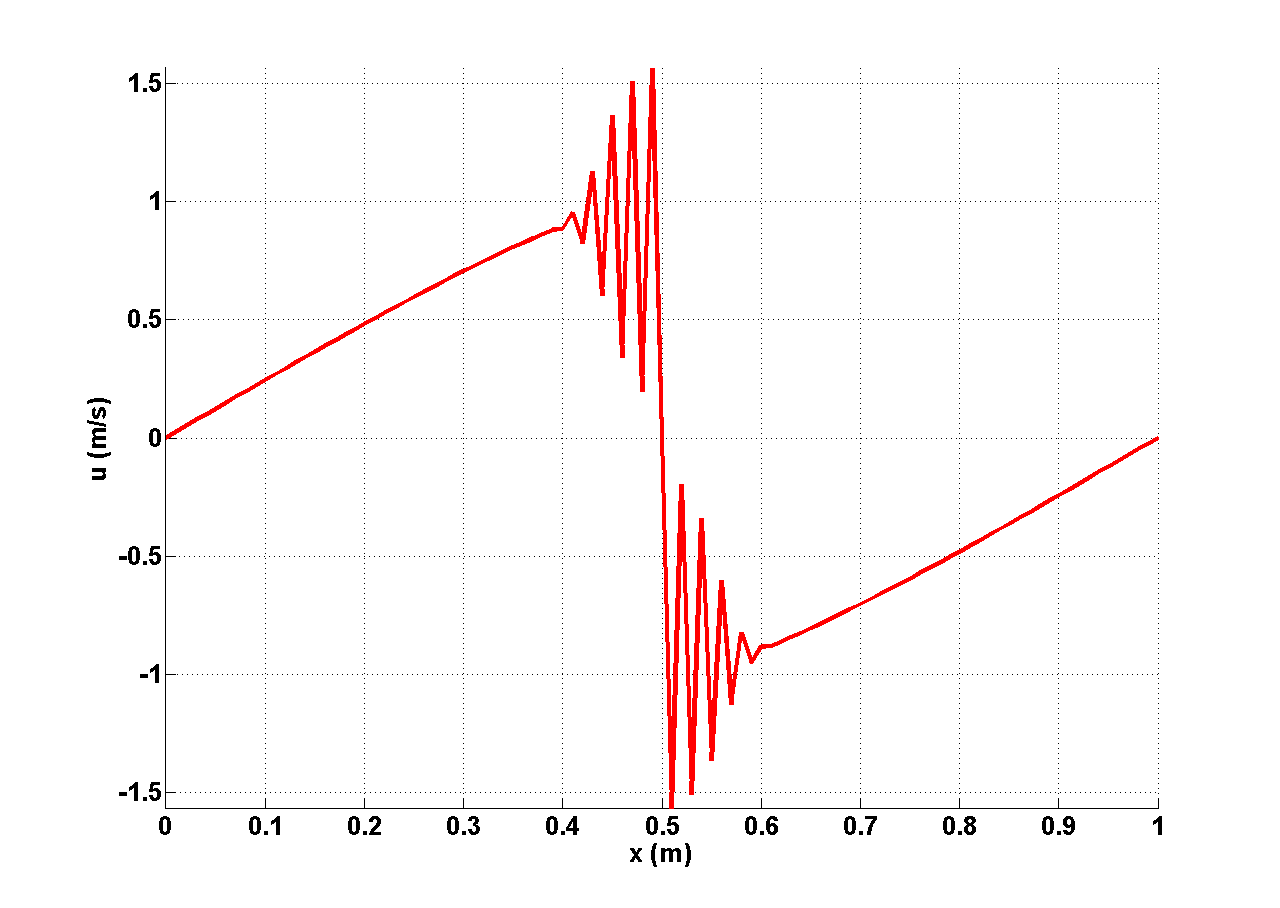
\includegraphics[width=\textwidth]{figs/1D_sol_free.png}
                \caption{Without stabilization.}
        \end{subfigure}%
        \begin{subfigure}[b]{0.37\textwidth}
                \centering
                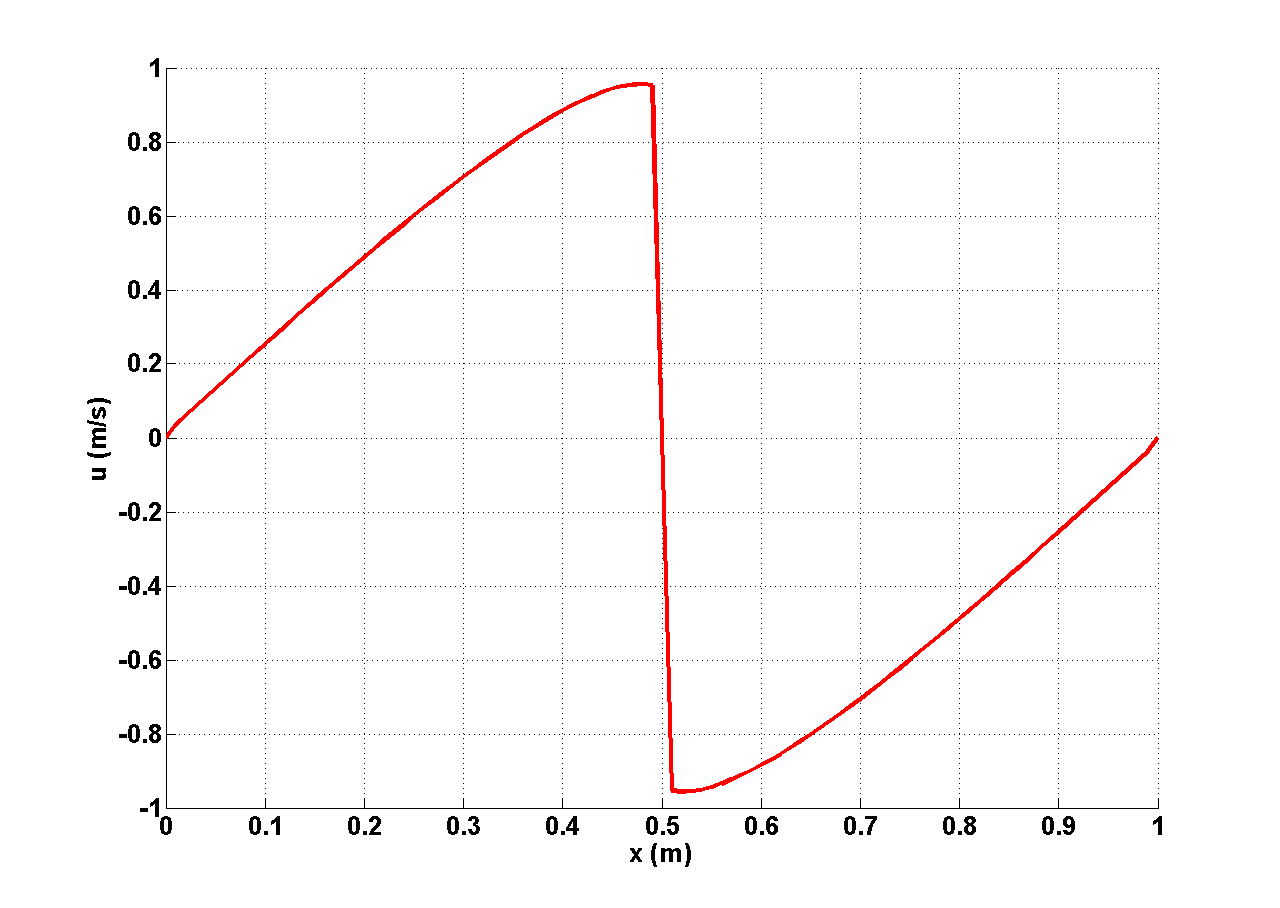
\includegraphics[width=\textwidth]{figs/1D_sol_fo.png}
                \caption{With first-order viscosity.}
        \end{subfigure}
        
        \begin{subfigure}[b]{0.37\textwidth}
                \centering
                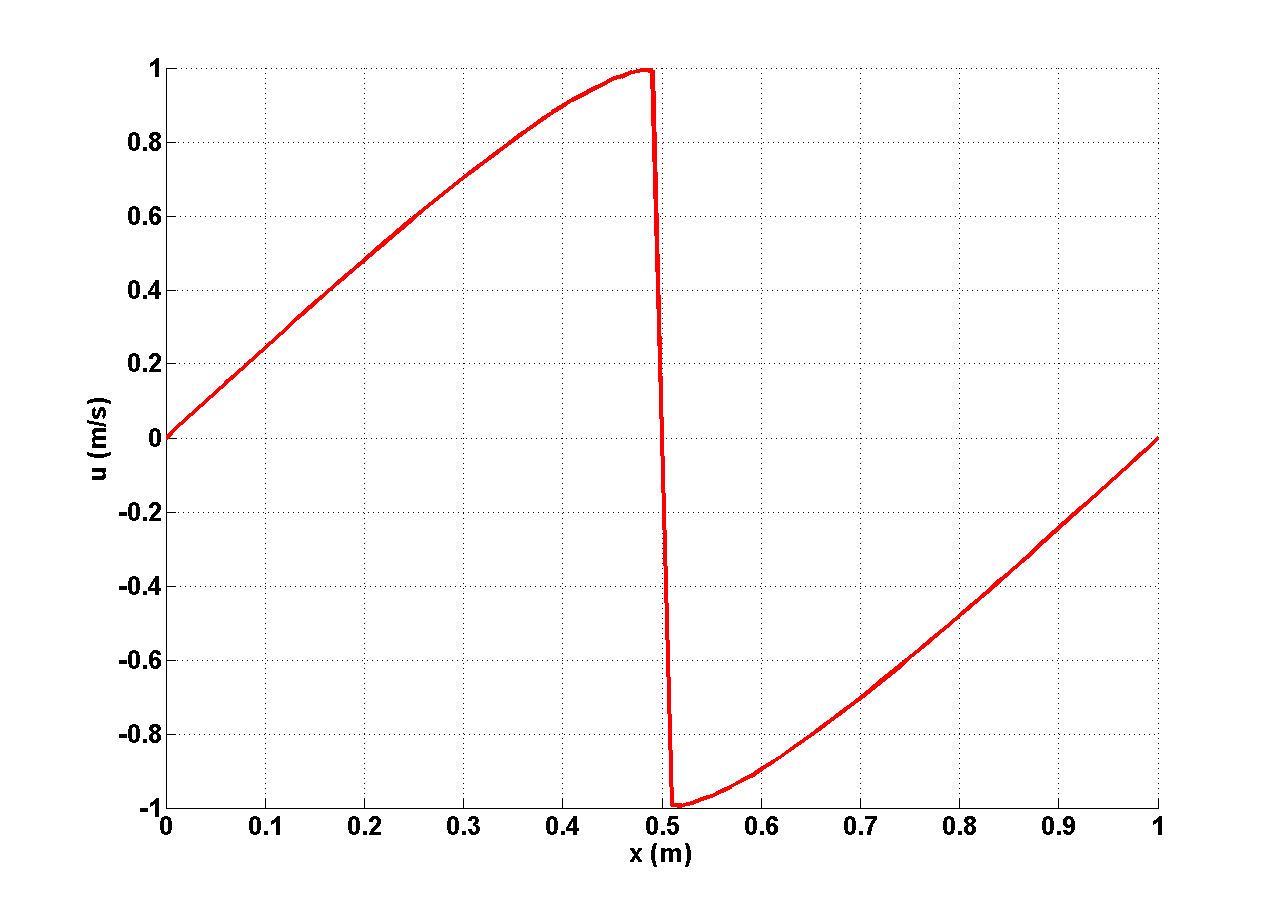
\includegraphics[width=\textwidth]{figs/1D_sol_ev.png}
                \caption{With the EVM.}
        \end{subfigure}
        \begin{subfigure}[b]{0.37\textwidth}
                \centering
                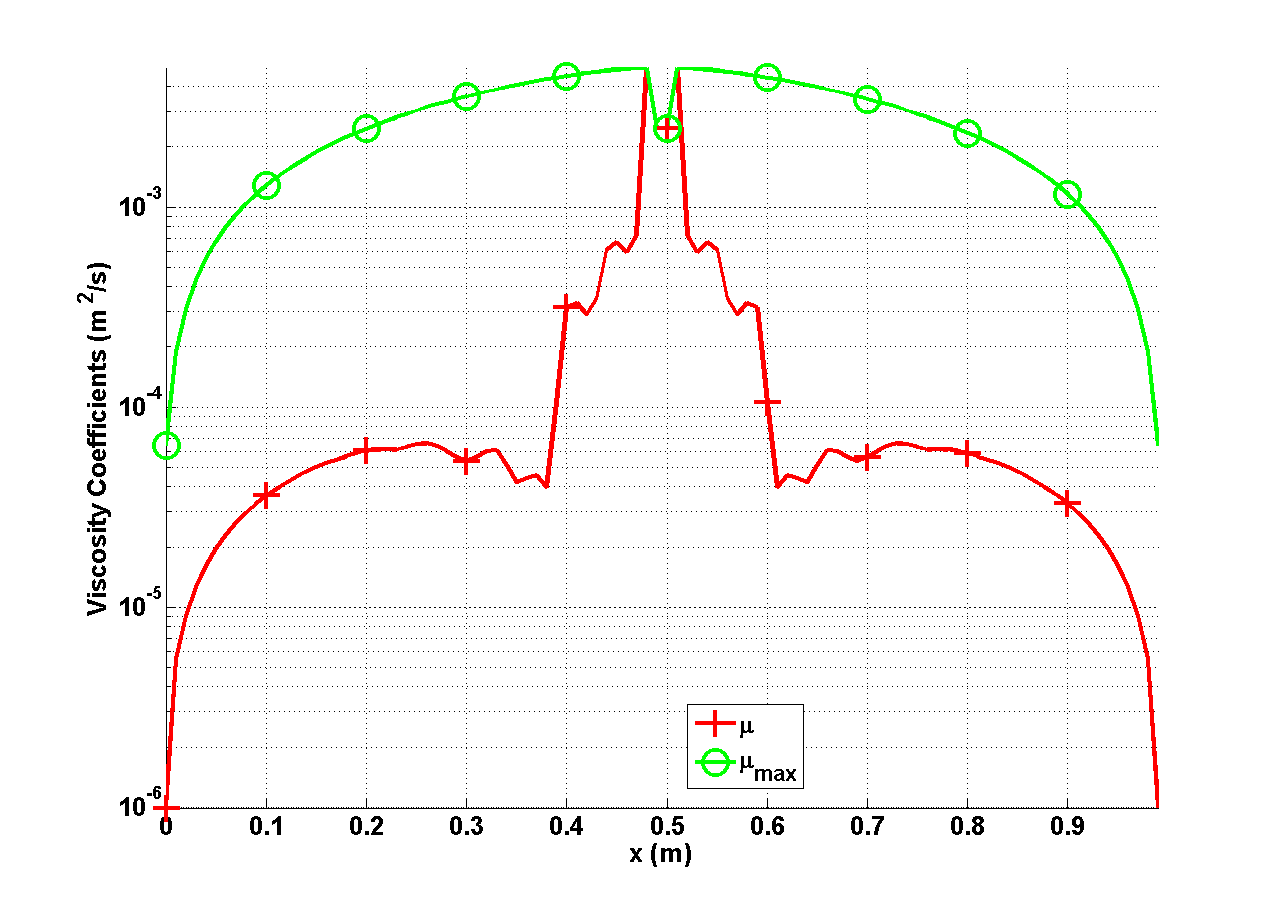
\includegraphics[width=\textwidth]{figs/1D_visc.png}
                \caption{Viscosity coefficient profiles.}
        \end{subfigure}
\end{figure}
\end{frame}
%%%%%%%%%%%%%%%%%%%%%%%%%%%%%%%%%%%%%%%%%%%%%%%%%%%%%%%%%%%%%%%%%%%%

%%%%%%%%%%%%%%%%%%%%%%%%%%%%%%%%%%%%%%%%%%%%%%%%%%%%%%%%%%%%%%%%%%%%
\subsection{Application to the Entropy Viscosity Method to the Euler Equations}
%%%%%%%%%%%%%%%%%%%%%%%%%%%%%%%%%%%%%%%%%%%%%%%%%%%%%%%%%%%%%%%%%%%%

%%%%%%%%%%%%%%%%%%%%%%%%%%%%%%%%%%%%%%%%%%%%%%%%%%%%%%%%%%%%%%%%%%%%
\begin{frame} 
\frametitle{Euler equations with viscous regularization}

\begin{block}{Eulers equations with viscous regularization}
\begin{subequations}
\label{eq:euler_visc_reg}
%
\begin{equation}
\partial_t \rho + \div \bs{m} - \tcr{\div \bs{f}} = 0
\end{equation}
%
\begin{equation}
\partial_t \bs{m} + \div (\bs{u} \otimes \bs{m}) + \grad p - \tcr{\div \mathbb{g}}  = 0
\end{equation}
%
\begin{equation}
\partial_t E + \div (\bs{u}(E+p)) - \tcr{\div (\bs{h}+ \mathbb{g} \cdot \bs{u} )}= 0
\end{equation}
%
\end{subequations}
+ Equation of State $P=P(\rho,e)$ %(here stiffened gas EOS)  $P = (\gamma-1) \rho (e-q) - \gamma P_\infty$
\end{block}

\medskip

The viscous fluxes $\bs{f}\,,\mathbb{g}\,,\bs{h}$ need to be determined. \textcolor{red}{How?} \\

\medskip

By proving that the equations with the regularization terms satisfy a minimum principle on the specific entropy:
\begin{block}{Minimum entropy principle}
\be
\inf_{x\in \mathbb{R}^d} s(x,t) \ge \inf_{x\in \mathbb{R}^d} s_0(x) \qquad \forall t \ge 0
\ee
\end{block}

\end{frame}

%%%%%%%%%%%%%%%%%%%%%%%%%%%%%%%%%%%%%%%%%%%%%%%%%%%%%%%%%%%%%%%%%%%%


%%%%%%%%%%%%%%%%%%%%%%%%%%%%%%%%%%%%%%%%%%%%%%%%%%%%%%%%%%%%%%%%%%%%
\begin{frame} 
\frametitle{}

\begin{block}{Euler equations with viscous regularization}
\begin{subequations}
\label{eq:euler_visc}
%
\begin{equation}
\partial_t \rho  + \div \left( \rho \vec{u} \right) = \textcolor{red}{\div \left( \kappa \grad \rho \right)} 
\end{equation}
%
\begin{equation}
\partial_t \left( \rho \vec{u} \right) + \div \left( \rho \vec{u} \otimes \vec{u} + P \mathbf{I} \right) = \textcolor{red}{\div \left( \mu \rho \grad^s \vec{u}  + \kappa \vec{u} \otimes \grad \rho \right) }
\end{equation}
%
\begin{equation}
\partial_t \left( \rho E \right) + \div \left[ \vec{u} \left( \rho E + P \right) \right] = \textcolor{red}{\div \left( \kappa \grad \left( \rho e \right) + \frac{1}{2}|| \vec{u} ||^2 \kappa \grad \rho +  \rho \mu \vec{u} \grad \vec{u}  \right) }
\end{equation}
\end{subequations}
where $\kappa$ and $\mu$ are positive viscosity coefficients.
\end{block}


\end{frame}
%%%%%%%%%%%%%%%%%%%%%%%%%%%%%%%%%%%%%%%%%%%%%%%%%%%%%%%%%%%%%%%%%%%%


%%%%%%%%%%%%%%%%%%%%%%%%%%%%%%%%%%%%%%%%%%%%%%%%%%%%%%%%%%%%%%%%%%%%
\begin{frame} 
\frametitle{Formulation (Guermond, 2011)}
\vspace{-3mm}
\begin{block}{\textcolor{red}{Entropy-based viscosity coefficients} $\kappa_e$ and $\mu_e$ :}
\begin{itemize}
\item are based on the local entropy production,  
\item are numerically \tcm{evaluated} using the local entropy residual $\resi(\vec{r},t) := \partial_t s + \vec{u} \cdot \grad s$ %
%\begin{equation}
%\label{eq:ent_residual}
%\resi(\vec{r}, t) := \partial_t s + \vec{u} \cdot \grad s
%\end{equation}
\end{itemize}
%
\begin{equation}
\longrightarrow
\quad \mu^K_e(\vec{r}_q,t) =  h_K^2 \frac{  |\resi^K(\vec{r}_q,t) |}{|| s - \bar{s} ||_\infty}  
\qquad 
\kappa^K_e(\vec{r}_q,t) = \Pr \, \mu^K_e(\vec{r}_q,t)
\end{equation}
%
% $\Pr$ is a user-defined parameter and is usually taken in the range $[ 0.001; 1 ]$.
%\medskip

The denominator $|| s - \bar{s} ||_\infty$ is used for dimensionality purposes,
\textcolor{magenta}{no theoretical justification beyond a dimensionality argument}
\end{block}

\vspace{-1mm}
\begin{block}{First-order viscosities}
We \tcb{determine the upper bounds} of these entropy-based viscosities by introducing the \textcolor{red}{first-order viscosity coefficients} $\mu_{\max}$ and $\kappa_{\max}$ :
%
\begin{equation}
\label{eq:fo}
\mu_{\max}(\vec{r}, t) = \kappa_{\max}(\vec{r}, t) = 0.5 h  \left( || \vec{u}(\vec{t,r}) || + c(\vec{t,r}) \right),
\end{equation}
If $\mu_{\max}$ and $\kappa_{\max}$ are used, the discretization scheme is over-dissipative and first-order.
\end{block}
%


\vspace{-1mm}
\begin{block}{Final definitions}
\be
\mu = \min (\mu_e , \mu_{\max}) \qquad \kappa = \min( \kappa_e , \kappa_{\max})
\ee
\end{block}

\end{frame}
%%%%%%%%%%%%%%%%%%%%%%%%%%%%%%%%%%%%%%%%%%%%%%%%%%%%%%%%%%%%%%%%%%%%


%%%%%%%%%%%%%%%%%%%%%%%%%%%%%%%%%%%%%%%%%%%%%%%%%%%%%%%%%%%%%%%%%%%%
%%%%%%%%%%%%%%%%%%%%%%%%%%%%%%%%%%%%%%%%%%%%%%%%%%%%%%%%%%%%%%%%%%%%
\section{Extension of the Entropy Viscosity Method to Low-Mach Flows}
%%%%%%%%%%%%%%%%%%%%%%%%%%%%%%%%%%%%%%%%%%%%%%%%%%%%%%%%%%%%%%%%%%%%
%%%%%%%%%%%%%%%%%%%%%%%%%%%%%%%%%%%%%%%%%%%%%%%%%%%%%%%%%%%%%%%%%%%%

%%%%%%%%%%%%%%%%%%%%%%%%%%%%%%%%%%%%%%%%%%%%%%%%%%%%%%%%%%%%%%%%%%%%
\subsection{New Formulation of the Entropy Residual}
%%%%%%%%%%%%%%%%%%%%%%%%%%%%%%%%%%%%%%%%%%%%%%%%%%%%%%%%%%%%%%%%%%%%


%%%%%%%%%%%%%%%%%%%%%%%%%%%%%%%%%%%%%%%%%%%%%%%%%%%%%%%%%%%%%%%%%%%%
\begin{frame} 
\frametitle{Low-Mach studies: New formulation for the entropy residual}

Recall that 

\begin{equation}
\mu^K_e(\vec{r}_q,t) =  h_K^2 \frac{|\resi^K(\vec{r}_q,t) |}{|| s - \bar{s} ||_\infty}  
\qquad
\kappa^K_e(\vec{r}_q,t) = \Pr \, \mu^K_e(\vec{r}_q,t)
\end{equation}


\begin{block}{Issues with current formulation in the low-Mach limit}
\begin{itemize}
\item In the low-Mach Regime, the flow is known to be \textcolor{red}{isentropic}, resulting in very little entropy production
\item In practice, the entropy residual $\resi$ will be very small in that regime  (i.e., small numerator in the expression for the viscosity coefficients)
\item and so will be the denominator $|| s - \bar{s} ||_\infty$,
\item Thus, the formula for the viscosity coefficients are not determined \textcolor{red}{(ill-scaled) in the low-Mach limit}
\end{itemize}
\end{block}

\end{frame}

%%%%%%%%%%%%%%%%%%%%%%%%%%%%%%%%%%%%%%%%%%%%%%%%%%%%%%%%%%%%%%%%%%%%

%%%%%%%%%%%%%%%%%%%%%%%%%%%%%%%%%%%%%%%%%%%%%%%%%%%%%%%%%%%%%%%%%%%%
\begin{frame} 
\frametitle{Alternate definition of the entropy residual}

%We can show that
\begin{equation}
\label{eq:ent_res}
\resi(\vec{r},t) := \partial_t s + \vec{u} \cdot \grad s = \matder{s} = \frac{s_e}{P_e} \underbrace{\left( \matder{P} - c^2 \matder{\rho} \right)}_{\resinew(\vec{r},t)} 
\end{equation} 

%Idea for the demonstration: 
%$s$ is a function of $e$ and $\rho$, thus $\matder{s} = s_e\matder{e} + s_\rho \matder{\rho}$\\
%Re-express the internal energy $e$ as a function of $P$ and $\rho$ through the EoS.

\begin{block}{Consequences}
\begin{itemize}
\item The entropy residuals $\resi$ and $\resinew$ are proportional to one another %and will experience similar variations in space and time. 
\item Thus, one may elect to employ $\resinew$ instead of $\resi$ %for the evaluation of the local entropy residual.
\item {\it An analytical expression of the entropy function $s$ is no longer needed} %: the residual $\resinew$ is evaluated using the local values of $P\,,\rho\,,u\,,c$ %pressure, density, velocity and speed of sound.
\item \textcolor{red}{Suitable normalizations for the residual} $\resinew$ can be devised (e.g., $P$, $\rho c^2$, $\rho c || \vec{u} ||$ or $\rho || \vec{u} ||^2$)%. Examples include the pressure itself or combinations of the density, the speed of sound and the norm of the velocity, i.e., $\rho c^2$, $\rho c || \vec{u} ||$ or $\rho || \vec{u} ||^2$. 
\end{itemize}
\end{block}


\begin{block}{What is the proper normalization for $\resinew(\vec{r},t)$?}
Requirements
\begin{enumerate}
\item To recover the incompressible results in the low-Mach limit %(i.e., pressure fluctuations $\propto M^2$; divergence-free flow; incompressible continuity equation)
\item To remain valid and accurate for supersonic flows
\end{enumerate}
\textcolor{red}{Asymptotic analysis} to determine the proper scaling in the low-Mach limit.

\end{block}

\end{frame}
%%%%%%%%%%%%%%%%%%%%%%%%%%%%%%%%%%%%%%%%%%%%%%%%%%%%%%%%%%%%%%%%%%%%



%%%%%%%%%%%%%%%%%%%%%%%%%%%%%%%%%%%%%%%%%%%%%%%%%%%%%%%%%%%%%%%%%%%%
\begin{frame} 
\frametitle{Bridging the gap from low-Mach to supersonic}

\begin{block}{Answer from low-Mach asymptotic study}
\begin{subequations}
\begin{equation}
\mu^K_e(\vec{r}_q,t)    = h_K^2 \frac{ | \resinew^K(\vec{r}_q,t) | }{ \rho_\infty c_\infty^2 }    \, ,
\end{equation} 
\text{and} 
\begin{equation}
\kappa^K_e(\vec{r}_q,t) = h_K^2 \frac{ | \resinew^K(\vec{r}_q,t) | }{ \rho_\infty c_\infty^2 } \, .
\end{equation}
\end{subequations}
\end{block}

However, we want to keep the all-speed aspect of the flow solver, so

\begin{block}{New definitions}
%\begin{subequations}
%\begin{equation}
%\mu^K_e(\vec{r},t)    = h_K^2 \frac{ | \resinew^K(\vec{r}_q,t) | }{\textcolor{magenta}{M \rho \|\vec{u}\|^2 + (1-M) \rho c^2}}  \, ,
%\end{equation} 
%\text{and} 
%\begin{equation}
%\kappa^K_e(\vec{r},t) = h_K^2 \frac{ | \resinew^K(\vec{r}_q,t) | }{\textcolor{magenta}{M \rho \|\vec{u}\|^2 + (1-M) \rho c^2}}  \, .
%\end{equation}
%\end{subequations}
%
%\underline{\textcolor{blue}{or, more generally,}}

\begin{subequations}
\begin{equation}
\mu^K_e(\vec{r},t)    = h_K^2 \frac{ | \resinew^K(\vec{r}_q,t) | }{\textcolor{magenta}{a(M) \rho \|\vec{u}\|^2 + (1-a(M)) \rho c^2}}  \, ,
\end{equation} 
\text{and} 
\begin{equation}
\kappa^K_e(\vec{r},t) = h_K^2 \frac{ | \resinew^K(\vec{r}_q,t) | }{\textcolor{magenta}{b(M) \rho \|\vec{u}\|^2 + (1-b(M)) \rho c^2}} \, .
\end{equation}
\end{subequations}

\end{block}

\end{frame}
%%%%%%%%%%%%%%%%%%%%%%%%%%%%%%%%%%%%%%%%%%%%%%%%%%%%%%%%%%%%%%%%%%%%



























%%%%%%%%%%%%%%%%%%%%%%%%%%%%%%%%%%%%%%%%%%%%%%%%%%%%%%%%%%%%%%%%%%%%
\subsection{Results}
%%%%%%%%%%%%%%%%%%%%%%%%%%%%%%%%%%%%%%%%%%%%%%%%%%%%%%%%%%%%%%%%%%%%

%%%%%%%%%%%%%%%%%%%%%%%%%%%%%%%%%%%%%%%%%%%%%%%%%%%%%%%%%%%%%%%%%%%%
\begin{frame} 
\frametitle{Numerical examples}

\bigskip 
All examples are obtained using MOOSE with linear continuous FEM (spatial discretization) and BDF2 (temporal integration).

\bigskip
Several shock tube examples available in the Appendix, if needed.
\end{frame}
%%%%%%%%%%%%%%%%%%%%%%%%%%%%%%%%%%%%%%%%%%%%%%%%%%%%%%%%%%%%%%%%%%%%

%%%%%%%%%%%%%%%%%%%%%%%%%%%%%%%%%%%%%%%%%%%%%%%%%%%%%%%%%%%%%%%%%%%%
\begin{frame} 
\frametitle{Mach-3 forward facing step: density contour}

\begin{center}
\movie[width=6cm,height=4cm,showcontrols=true,externalviewer]{
\includegraphics[width=6cm,height=4cm]{engr.pdf}}{movs/forward_facing_step_density_movie.mpeg}\\
\end{center}

%\begin{center}
  %\begin{columns}
    %\column{.5\textwidth}
       %\includemedia[addresource=compression_corner.mp4, activate=pageopen, deactivate=pageclose, width=6.5cm, height=5cm, flashvars={source=mov/compression_corner.mp4 & autoPlay=true & loop=true }]{}{VPlayer.swf}
    %\column{.5\textwidth}
      %\includemedia[addresource=compression_corner_viscosity.mp4, activate=pageopen, deactivate=pageclose, width=6.5cm, height=5cm, flashvars={source=mov/compression_corner_viscosity.mp4 & autoPlay=true & loop=true }]{}{VPlayer.swf}
  %\end{columns}
%\end{center}


\end{frame}
\begin{frame} 
\frametitle{Mach-3 forward facing step: viscosity contour}

\begin{center}
\movie[width=6cm,height=4cm,showcontrols=true,externalviewer]{
\includegraphics[width=6cm,height=4cm]{engr.pdf}}{movs/forward_facing_step_viscosity.mpeg}\\
\end{center}

\end{frame}
%%%%%%%%%%%%%%%%%%%%%%%%%%%%%%%%%%%%%%%%%%%%%%%%%%%%%%%%%%%%%%%%%%%%

%%%%%%%%%%%%%%%%%%%%%%%%%%%%%%%%%%%%%%%%%%%%%%%%%%%%%%%%%%%%%%%%%%%%
%%%%%%%%%%%%%%%%%%%%%%%%%%%%%%%%%%%%%%%%%%%%%%%%%%%%%%%%%%%%%%%%%%%%
\section{Extension of the Entropy Viscosity Method to Low-Mach Flows}
%%%%%%%%%%%%%%%%%%%%%%%%%%%%%%%%%%%%%%%%%%%%%%%%%%%%%%%%%%%%%%%%%%%%
%%%%%%%%%%%%%%%%%%%%%%%%%%%%%%%%%%%%%%%%%%%%%%%%%%%%%%%%%%%%%%%%%%%%

%%%%%%%%%%%%%%%%%%%%%%%%%%%%%%%%%%%%%%%%%%%%%%%%%%%%%%%%%%%%%%%%%%%%
\subsection{New formulation for the entropy residual}
%%%%%%%%%%%%%%%%%%%%%%%%%%%%%%%%%%%%%%%%%%%%%%%%%%%%%%%%%%%%%%%%%%%%


%%%%%%%%%%%%%%%%%%%%%%%%%%%%%%%%%%%%%%%%%%%%%%%%%%%%%%%%%%%%%%%%%%%%
\begin{frame} 
\frametitle{Low-Mach studies: New formulation for the entropy residual}

Recall that 
\begin{subequations}
\begin{equation}
\mu^K_e(\vec{r}_q,t) =  h_K^2 \frac{|\resi^K(\vec{r}_q,t) |}{|| s - \bar{s} ||_\infty}  
\end{equation}
\begin{equation}
\kappa^K_e(\vec{r}_q,t) = \Pr \, \mu^K_e(\vec{r}_q,t)
\end{equation}
\end{subequations}


\begin{block}{Issue with current formulation in the low-Mach limit}
\begin{itemize}
\item In the low-Mach Regime, the flow is known to be \textcolor{red}{isentropic}, resulting in very little entropy production
\item In practice, the entropy residual $\resi$ will be very small in that regime  (i.e., small numerator in the expression for the viscosity coefficients)
\item and so will be the denominator $|| s - \bar{s} ||_\infty$,
\item Thus, the formula for the viscosity coefficients are not determined \textcolor{red}{(ill-scaled) in the low-Mach limit}
\end{itemize}
\end{block}

\end{frame}

%%%%%%%%%%%%%%%%%%%%%%%%%%%%%%%%%%%%%%%%%%%%%%%%%%%%%%%%%%%%%%%%%%%%

%%%%%%%%%%%%%%%%%%%%%%%%%%%%%%%%%%%%%%%%%%%%%%%%%%%%%%%%%%%%%%%%%%%%
\begin{frame} 
\frametitle{Alternate definition of the entropy residual}

\begin{equation}
\label{eq:ent_res}
\resi(\vec{r},t) := \partial_t s + \vec{u} \cdot \grad s = \matder{s} = \frac{s_e}{P_e} \left( \underbrace{\matder{P} - c^2 \matder{\rho} }_{\resinew(\vec{r},t)} \right) ,
\end{equation} 

Idea for the demonstration: 
$s$ is a function of $e$ and $\rho$, thus $\matder{s} = s_e\matder{e} + s_\rho \matder{\rho}$\\
Re-express the internal energy $e$ as a function of $P$ and $\rho$ through the EoS.

\begin{block}{Outcome}
\begin{itemize}
\item The entropy residuals $\resi$ and $\resinew$ are proportional to one another and will experience similar variations in space and time. 
\item Thus, one may elect to employ $\resinew$ instead of $\resi$ %for the evaluation of the local entropy residual.
\item {\it An analytical expression of the entropy function $s$ is no longer needed}: the residual $\resinew$ is evaluated using the local values of $P\,,\rho\,,u\,,c$ %pressure, density, velocity and speed of sound.
\item \textcolor{red}{Suitable normalizations for the residual} $\resinew$ can be devised. Examples include the pressure itself or combinations of the density, the speed of sound and the norm of the velocity, i.e., $\rho c^2$, $\rho c || \vec{u} ||$ or $\rho || \vec{u} ||^2$. 
\end{itemize}
\end{block}

\end{frame}
%%%%%%%%%%%%%%%%%%%%%%%%%%%%%%%%%%%%%%%%%%%%%%%%%%%%%%%%%%%%%%%%%%%%

%%%%%%%%%%%%%%%%%%%%%%%%%%%%%%%%%%%%%%%%%%%%%%%%%%%%%%%%%%%%%%%%%%%%
\begin{frame} 
\frametitle{New definition for the entropy viscosity coefficients}

Let's pose
\begin{subequations}
\label{eq:visc_definition}
\begin{equation}
\mu^K_e(\vec{r}_q,t)    = h_K^2 \frac{ | \resinew^K(\vec{r}_q,t) | }{\norm_P^\mu}    \, ,
\end{equation} 
\text{and} 
\begin{equation}
\kappa^K_e(\vec{r}_q,t) = h_K^2 \frac{ | \resinew^K(\vec{r}_q,t) | }{\norm_P^\kappa} \, .
\end{equation}
\end{subequations}

\bigskip

We now need to determine $\norm_P^\mu$ and $\norm_P^\kappa$.

\bigskip

\textcolor{red}{Asymptotic analysis} to determine the viscosity coefficient scaling in the low-Mach limit.

\end{frame}
%%%%%%%%%%%%%%%%%%%%%%%%%%%%%%%%%%%%%%%%%%%%%%%%%%%%%%%%%%%%%%%%%%%%

%%%%%%%%%%%%%%%%%%%%%%%%%%%%%%%%%%%%%%%%%%%%%%%%%%%%%%%%%%%%%%%%%%%%
\subsection{Asymptotic and more}
%%%%%%%%%%%%%%%%%%%%%%%%%%%%%%%%%%%%%%%%%%%%%%%%%%%%%%%%%%%%%%%%%%%%

%%%%%%%%%%%%%%%%%%%%%%%%%%%%%%%%%%%%%%%%%%%%%%%%%%%%%%%%%%%%%%%%%%%%
\begin{frame} 
\frametitle{Dimensionless variables}

\begin{multline}
\label{eq:norm_param}
\rho^*   = \frac{\rho}{\rho_\infty}           ,\
u^*      = \frac{u}{u_\infty}                 ,\
P^*      = \frac{P}{\rho_\infty c^2_\infty}   ,\
E^*      = \frac{E}{c^2_\infty }              ,\\
x^* = \frac{x}{L_\infty}                      ,\
t^* = \frac{t}{L_\infty / u_\infty}           ,\ 
\mu^*    = \frac{\mu}{\mu_\infty}             ,\
\kappa^* = \frac{\kappa}{\kappa_\infty}       ,
\end{multline}
%
where  the subscript $\infty$ denote the far-field or stagnation quantities and the superscript $*$ stands for the adimensional variables.

\medskip

The far-field reference quantities are chosen such that the dimensionless flow quantities are of order 1. 

\medskip

The reference Mach number is given by
%
\begin{equation}
M_\infty = \frac{u_\infty}{c_\infty} ,
\end{equation}

\end{frame}
%%%%%%%%%%%%%%%%%%%%%%%%%%%%%%%%%%%%%%%%%%%%%%%%%%%%%%%%%%%%%%%%%%%%

%%%%%%%%%%%%%%%%%%%%%%%%%%%%%%%%%%%%%%%%%%%%%%%%%%%%%%%%%%%%%%%%%%%%
\begin{frame} 
\frametitle{Scaled Euler equations with viscous regularization}

\begin{subequations} 
\label{eq:Euler_eq2}
%
\begin{equation}
\label{eq:euler_eq2_cont}
\partial_{t^*} \rho^*+ \divv{*}  \left(  \rho^* \vec{u}^*  \right) = \frac{1}{\tcr{\Pe_\infty}} \divv{*}  ( \kappa^* \gradd{*} \rho^* )
\end{equation}
%
\begin{multline}
\label{eq:euler_eq2_mom}
\partial_{t^*} \left( \rho^* \vec{u}^* \right) 
+ \divv{*} \left( \rho^* \vec{u}^*\otimes \vec{u}^* \right) 
+ \frac{1}{\tcr{M_\infty^2}}\gradd{*}  P^*  
= 
\frac{1}{\tcr{\Re_\infty}} \divv{*} \left( \rho^* \mu^* \gradd{s,*} \vec{u}^* \right)  \\
+
\frac{1}{\tcr{\Pe_\infty}} \divv{*} \left(\vec{u}^*\otimes \kappa^* \gradd{*}  \rho^* \right)
\end{multline}
%
\begin{multline}
\label{eq:euler_eq2_energy}
\partial_{t^*} \left( \rho^* E^* \right) 
+ \divv{*}  \left[ \vec{u}^* \left( \rho^* E^* + P^* \right) \right] 
=
\frac{1}{\tcr{\Pe_\infty}} \divv{*}  \left( \kappa^*  \gradd{*} (\rho^* e^*) \right)   \\
+
\frac{M_\infty^2}{\Re_\infty} \divv{*}  \left( \vec{u}^* \rho^* \mu^* \gradd{s,*} \vec{u}^* \right)
+ 
\frac{M_\infty^2}{2 \Pe_\infty} \divv{*}  \left(\kappa^* (u^*)^2 \gradd{*} \rho^* \right) \, ,
\end{multline}
%
\end{subequations}

\medskip

where the numerical Reynolds $(\Re_\infty)$ and P\'eclet $(\Pe_\infty)$ numbers are :
%
\begin{equation}
\label{eq:ref_numb}
\Re_\infty = \frac{u_\infty L_\infty}{\mu_\infty} \text{ and }
\Pe_\infty = \frac{u_\infty L_\infty}{\kappa_\infty} \, .
\end{equation}
%
%The Prandlt number used in the original version of the method is simply given by 
%\begin{equation} \label{eq:ref_nb_pr} 
%\Pr_\infty = \Pe_\infty / \Re_\infty \, .
%\end{equation}

\end{frame}
%%%%%%%%%%%%%%%%%%%%%%%%%%%%%%%%%%%%%%%%%%%%%%%%%%%%%%%%%%%%%%%%%%%%

%%%%%%%%%%%%%%%%%%%%%%%%%%%%%%%%%%%%%%%%%%%%%%%%%%%%%%%%%%%%%%%%%%%%
\begin{frame} 
\frametitle{How should $\Re$ and $\Pe$ scale with the Mach number???}

Expand each variable in powers of the Mach number. As an example, 
%
\begin{equation}
\label{eq:expansion}
P(\vec{r}, t) = P_0(\vec{r}, t) + P_1(\vec{r}, t) M_\infty + P_2(\vec{r}, t) M_\infty^2 + \dots 
\end{equation}

By studying the resulting momentum equations for various powers of $M_\infty$, we observe the following: the leading order and first-order pressure terms, $P_0$ and $P_1$, are spatially constant \textcolor{magenta}{if and only if} $\Re_\infty = \Pe_\infty = 1$. 


In this case, the leading-order expressions for the continuity, momentum, and energy equations are:
\begin{subequations}
\label{eq:asympt_equ2}
%
\begin{equation}
\label{eq:asympt_equ2_cont}
 \partial_t \rho_0 + \div ( \rho \vec{u} )_0 = \div ( \kappa \grad \rho )_0
\end{equation}
%
\begin{equation}
\label{eq:asympt_equ2_mom}
\partial_t (\rho \vec{u})_0 + \div ( \rho \vec{u} \otimes \vec{u})_0 + \grad P_2 = \div (\rho \mu \grad^s \vec{u} +\kappa \vec{u} \otimes \grad \rho )_0
\end{equation}
%
\begin{equation}
\label{eq:asympt_equ2_ener}
 \partial_t(\rho E)_0 + \div \left[ \vec{u} (\rho E + P) \right]_0 = \div(\kappa \grad(\rho e))_0
\end{equation}
%
\end{subequations}

This is consistent with the \textcolor{magenta}{the results in the incompressible limit}

\end{frame}
%%%%%%%%%%%%%%%%%%%%%%%%%%%%%%%%%%%%%%%%%%%%%%%%%%%%%%%%%%%%%%%%%%%%

%%%%%%%%%%%%%%%%%%%%%%%%%%%%%%%%%%%%%%%%%%%%%%%%%%%%%%%%%%%%%%%%%%%%
\begin{frame} 
%\frametitle{}
The leading-order of the equation of state is given by 
\begin{equation}
\label{eq:leading_order_eos}
 P_0 = (\gamma - 1) (\rho E)_0 .
\end{equation}
%
Using \eqt{eq:leading_order_eos}, the energy equation can be recast as a function of the leading-order pressure, $P_0$, as follows:
%
\begin{equation}\label{eq:asympt_equ3_ener}
 \partial_t P_0 + \gamma \div \left( \vec{u} P \right)_0 =  \div(\kappa \grad(P))_0
\end{equation}
%
Since $P_0$ is spatially constant, \eqt{eq:asympt_equ3_ener} becomes
%
\begin{equation}
\frac{1}{\gamma P_0} \frac{d P_0}{dt} = - \div \vec{u}_0 
\end{equation}
%
and, at steady state, we have
%
\begin{equation}
% \gamma P_0 \div  \vec{u}_0 = 0 \Rightarrow \div  \vec{u}_0 = 0.
 \div  \vec{u}_0 = 0 \, .
\end{equation}


The same reasoning can be applied to the leading-order of the continuity equation to show that
\begin{equation}
\matder{\rho_0} := \partial_t \rho_0 + \vec{u}_0 \cdot \div \rho_0 = 0 \, .
\end{equation}
%
Therefore, by setting the $\Re=\Pe=1$, the \tcr{incompressible fluid results are retrieved in the low-Mach limit when employing the compressible Euler equations with viscous regularization terms present}.


\end{frame}
%%%%%%%%%%%%%%%%%%%%%%%%%%%%%%%%%%%%%%%%%%%%%%%%%%%%%%%%%%%%%%%%%%%%


%%%%%%%%%%%%%%%%%%%%%%%%%%%%%%%%%%%%%%%%%%%%%%%%%%%%%%%%%%%%%%%%%%%%
\begin{frame} 
\frametitle{Back to $\norm_P^\mu$ and $\norm_P^\kappa$}

From the definition of the entropy viscosity coefficient, we have
\begin{equation}
\label{eq:norm_relation}
\kappa_\infty 
= \frac{ \rho_\infty c_\infty^2 L_\infty^2 }{ L_\infty/u_\infty  \norm_{P,\infty}^{\kappa} }
= \frac{ \rho_\infty c_\infty^2 u_\infty L_\infty }{ \norm_{P,\infty}^{\kappa} } \, .
\end{equation}

Since $\Pe$ scales as unity,  we obtain:
%
\begin{equation}
\label{eq:norm_relation_bis}
\norm_{P,\infty}^{\kappa} = \Pe_\infty \rho_\infty c_\infty^2 = \rho_\infty c_\infty^2 \, .
\end{equation}
%
\eqt{eq:norm_relation_bis} provides a proper normalization factor to define the $\kappa$ viscosity coefficient.\\

\medskip 
Similarly :  $\norm_{P,\infty}^{\mu} = \rho_\infty c_\infty^2 $.

\begin{block}{Thus, some possible new definitions in the low-Mach limit are}
\begin{subequations}
\begin{equation}
\mu^K_e(\vec{r}_q,t)    = h_K^2 \frac{ | \resinew^K(\vec{r}_q,t) | }{ \rho_\infty c_\infty^2 }    \, ,
\end{equation} 
\text{and} 
\begin{equation}
\kappa^K_e(\vec{r}_q,t) = h_K^2 \frac{ | \resinew^K(\vec{r}_q,t) | }{ \rho_\infty c_\infty^2 } \, .
\end{equation}
\end{subequations}
\end{block}

\end{frame}
%%%%%%%%%%%%%%%%%%%%%%%%%%%%%%%%%%%%%%%%%%%%%%%%%%%%%%%%%%%%%%%%%%%%


%%%%%%%%%%%%%%%%%%%%%%%%%%%%%%%%%%%%%%%%%%%%%%%%%%%%%%%%%%%%%%%%%%%%
\begin{frame} 
\frametitle{Bridging the gap from low-Mach to supersonic}

However, we want to keep the all-speed aspect of the flow solver, so

\begin{block}{New definitions}
\begin{subequations}
\begin{equation}
\mu^K_e(\vec{r},t)    = h_K^2 \frac{ | \resinew^K(\vec{r}_q,t) | }{\textcolor{magenta}{M \rho \|\vec{u}\|^2 + (1-M) \rho c^2}}  \, ,
\end{equation} 
\text{and} 
\begin{equation}
\kappa^K_e(\vec{r},t) = h_K^2 \frac{ | \resinew^K(\vec{r}_q,t) | }{\textcolor{magenta}{M \rho \|\vec{u}\|^2 + (1-M) \rho c^2}}  \, .
\end{equation}
\end{subequations}

\underline{\textcolor{blue}{or, more generally,}}

\begin{subequations}
\begin{equation}
\mu^K_e(\vec{r},t)    = h_K^2 \frac{ | \resinew^K(\vec{r}_q,t) | }{\textcolor{magenta}{a(M) \rho \|\vec{u}\|^2 + (1-a(M)) \rho c^2}}  \, ,
\end{equation} 
\text{and} 
\begin{equation}
\kappa^K_e(\vec{r},t) = h_K^2 \frac{ | \resinew^K(\vec{r}_q,t) | }{\textcolor{magenta}{b(M) \rho \|\vec{u}\|^2 + (1-b(M)) \rho c^2}}  \, .
\end{equation}
\end{subequations}

\end{block}

\end{frame}
%%%%%%%%%%%%%%%%%%%%%%%%%%%%%%%%%%%%%%%%%%%%%%%%%%%%%%%%%%%%%%%%%%%%
















%%%%%%%%%%%%%%%%%%%%%%%%%%%%%%%%%%%%%%%%%%%%%%%%%%%%%%%%%%%%%%%%%%%%
\subsection{Numerical Results}
%%%%%%%%%%%%%%%%%%%%%%%%%%%%%%%%%%%%%%%%%%%%%%%%%%%%%%%%%%%%%%%%%%%%


%%%%%%%%%%%%%%%%%%%%%%%%%%%%%%%%%%%%%%%%%%%%%%%%%%%%%%%%%%%%%%%%%%%%
\begin{frame} 
%\frametitle{Fluid flow over a 2-D cylinder at various inlet Mach values (CFL=40)}
\frametitle{Fluid flow over a 2-D cylinder with an inlet Mach of $10^{-3}$ (CFL=40)}

%At steady state:
\begin{figure}
	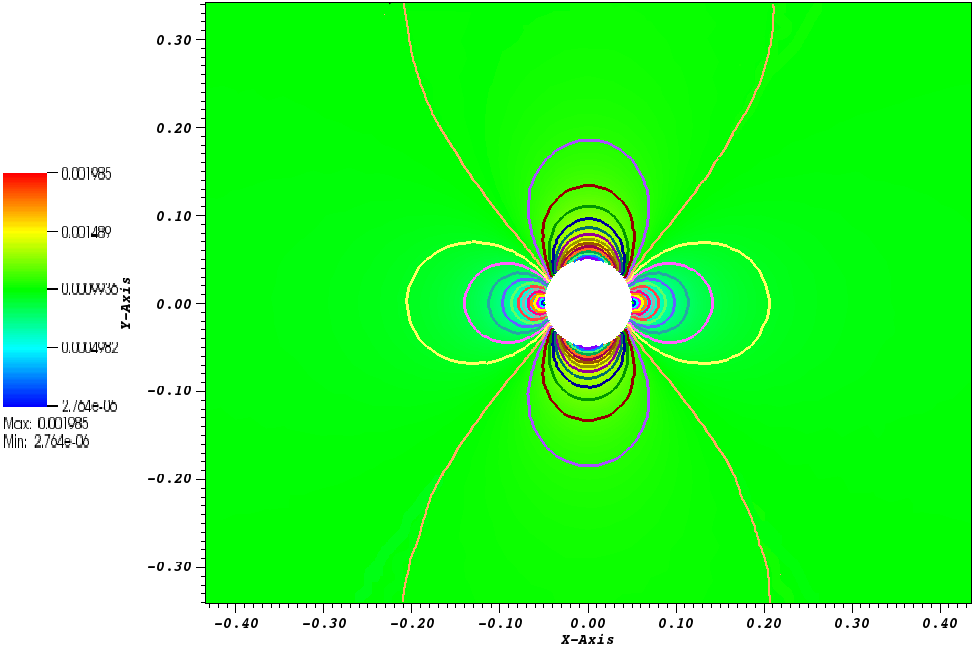
\includegraphics[height=6cm, keepaspectratio=true]{figs/CylinderMach1em3ZoomIn.png}
  \caption{$M_{\text{inlet}}=10^{-3}$}
\end{figure}
\end{frame}
%
%\begin{frame} 
%\begin{figure}
	%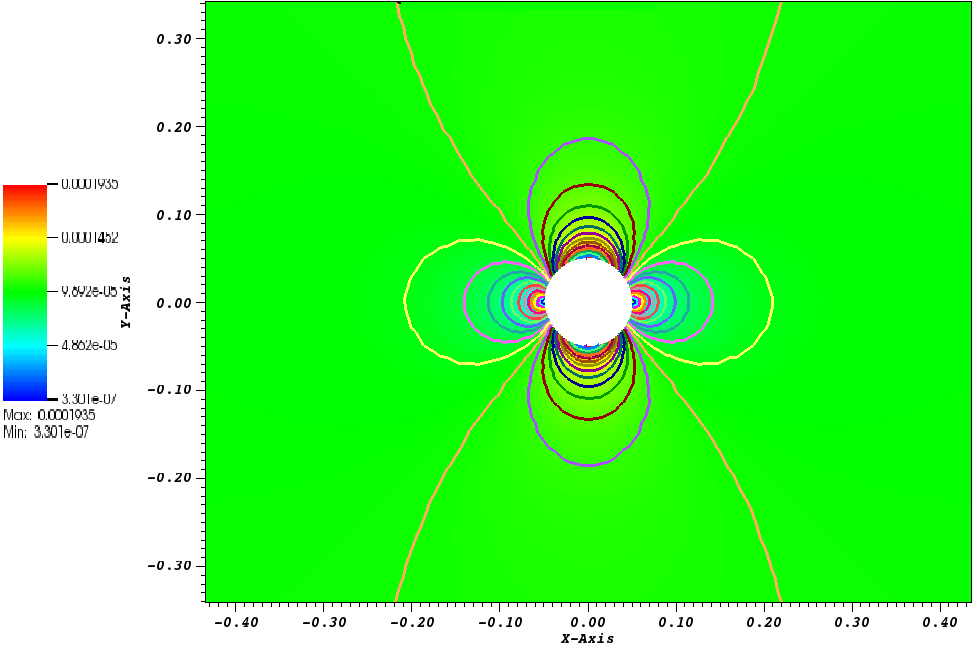
\includegraphics[height=7cm, keepaspectratio=true]{figs/CylinderMach1em4ZoomIn.png}
  %\caption{$M_{\text{inlet}}=10^{-4}$}
%\end{figure}
%\end{frame}
%
%\begin{frame} 
%\begin{figure}
	%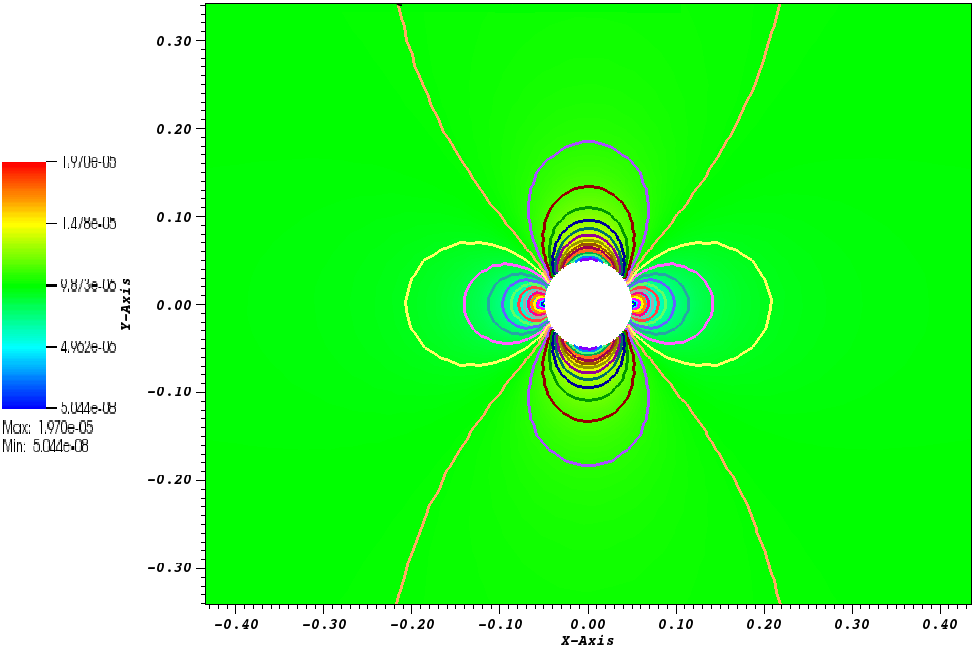
\includegraphics[height=7cm, keepaspectratio=true]{figs/CylinderMach1em5ZoomIn.png}
  %\caption{$M_{\text{inlet}}=10^{-5}$}
%\end{figure}
%\end{frame}
%
%\begin{frame} 
%\begin{figure}
	%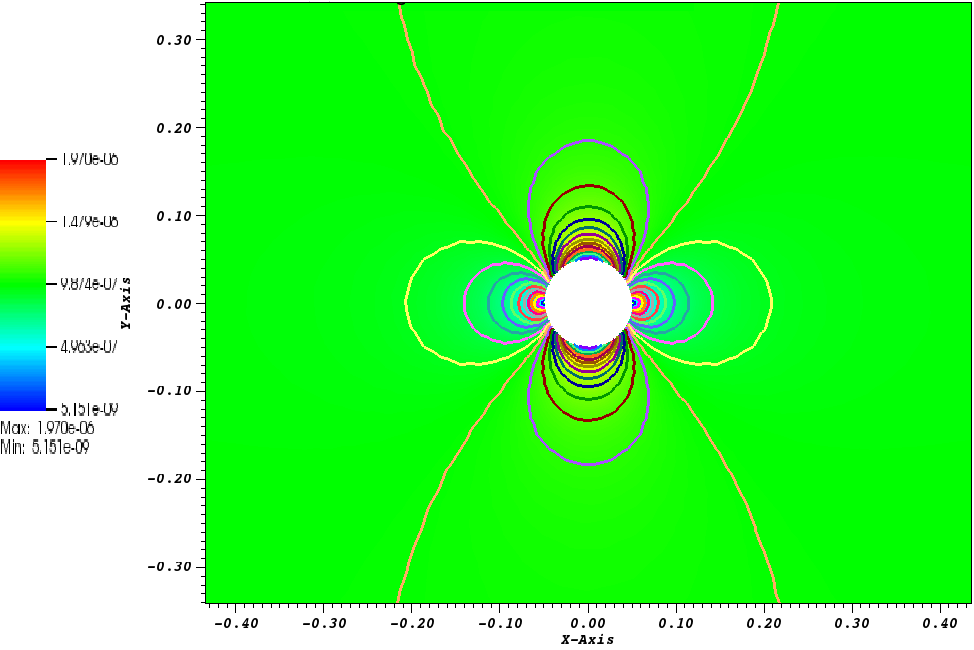
\includegraphics[height=7cm, keepaspectratio=true]{figs/CylinderMach1em6ZoomIn.png}
  %\caption{$M_{\text{inlet}}=10^{-6}$}
%\end{figure}
%\end{frame}
%
\begin{frame} 
\frametitle{Fluid flow over a 2-D cylinder with an inlet Mach of $10^{-7}$ (CFL=40)}

\begin{figure}
	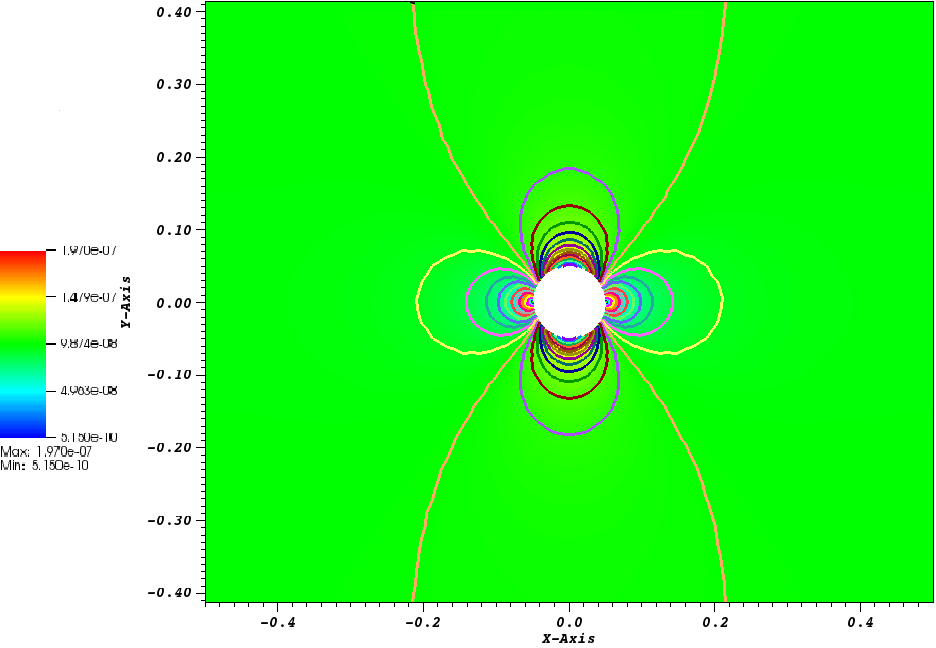
\includegraphics[height=7cm, keepaspectratio=true]{figs/CylinderMach1em7ZoomIn.png}
  \caption{$M_{\text{inlet}}=10^{-7}$}
\end{figure}
\end{frame}

\begin{frame}{}Velocity ratio for different Mach numbers}
\begin{table}[H]
\begin{center}
 \caption{\label{tbl:velocity_ratio}Velocity ratio for different Mach numbers.}
\begin{tabular}{|c|c|c|c|}
\hline
Mach number & inlet velocity & velocity at the top of the cylinder & ratio \\ \hline
$10^{-3}$ & $2.348$ $10^{-3}$ & $1.176$ $10^{-3}$& $1.99$  \\ \hline
$10^{-4}$ & $2.285$ $10^{-4}$ & $1.145$ $10^{-4}$& $1.99$  \\ \hline
$10^{-5}$ & $2.283$ $10^{-5}$ & $1.144$ $10^{-5}$ & $1.99$ \\ \hline
$10^{-6}$ & $2.283$ $10^{-6}$ & $1.144$ $10^{-6}$ & $1.99$ \\ \hline
$10^{-7}$ & $2.283$ $10^{-7}$ & $1.144$ $10^{-7}$ & $1.99$ \\ \hline
\end{tabular}
\end{center}
\nonumber
\end{table}
\end{frame}


\begin{frame}{Pressure and velocity fluctuations versus $M$}
\begin{figure}
	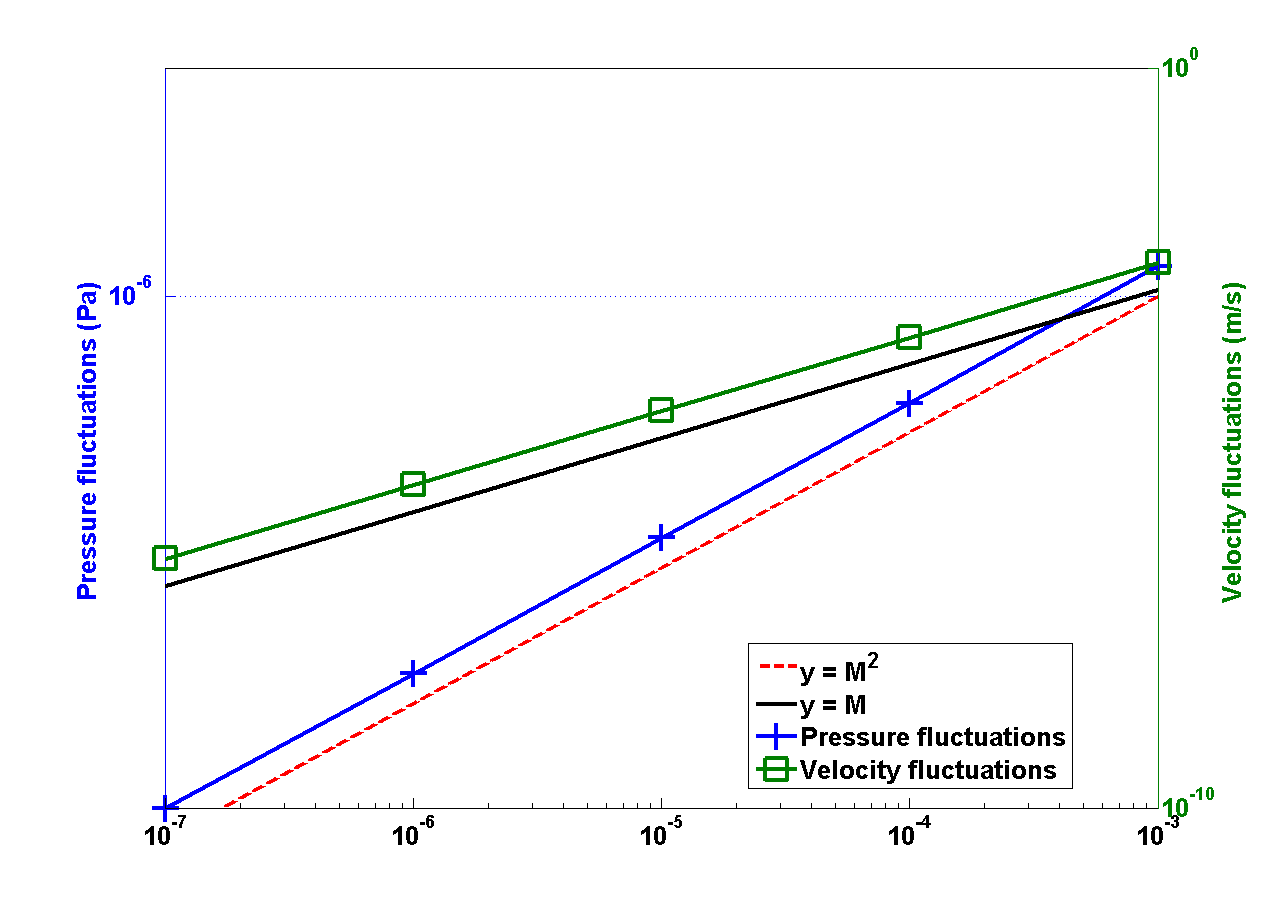
\includegraphics[height=7cm, keepaspectratio=true]{figs/pressure_fluctuation.png}
\end{figure}
\end{frame}

%%%%%%%%%%%%%%%%%%%%%%%%%%%%%%%%%%%%%%%%%%%%%%%%%%%%%%%%%%%%%%%%%%%%%


%%%%%%%%%%%%%%%%%%%%%%%%%%%%%%%%%%%%%%%%%%%%%%%%%%%%%%%%%%%%%%%%%%%%
\begin{frame} 
\frametitle{Flow over a circular hump (CFL=20)}

At steady state:
\begin{figure}
	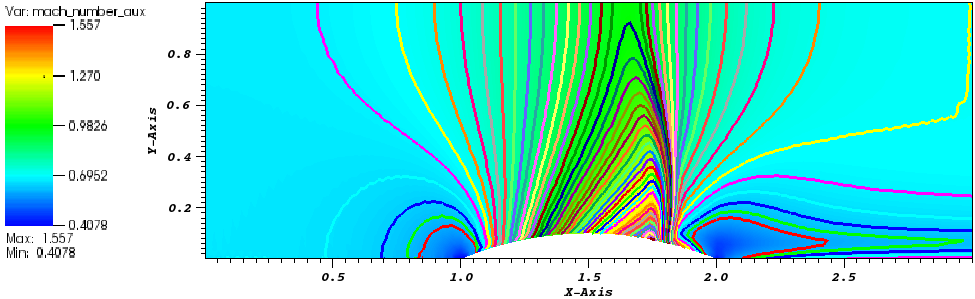
\includegraphics[height=3cm, keepaspectratio=true]{figs/Hump2D_mach_0p7.png}
  \caption{$M_{\text{inlet}}=0.7$}
\end{figure}
\end{frame}

\begin{frame} 
\begin{figure}
	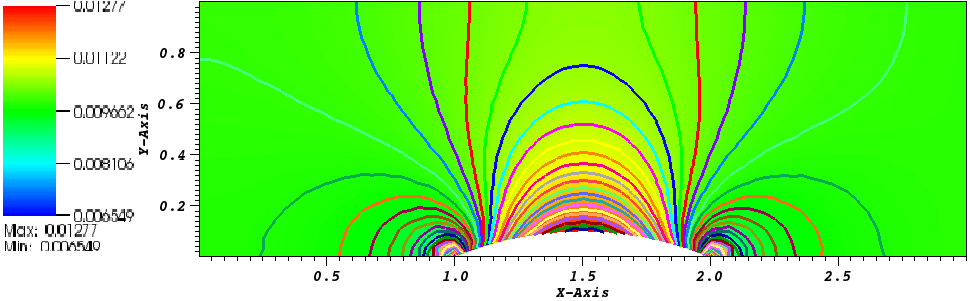
\includegraphics[height=3cm, keepaspectratio=true]{figs/Hump2D_mach_0p01.png}
  \caption{$M_{\text{inlet}}=10^{-2}$}
\end{figure}
\end{frame}

\begin{frame} 
\begin{figure}
	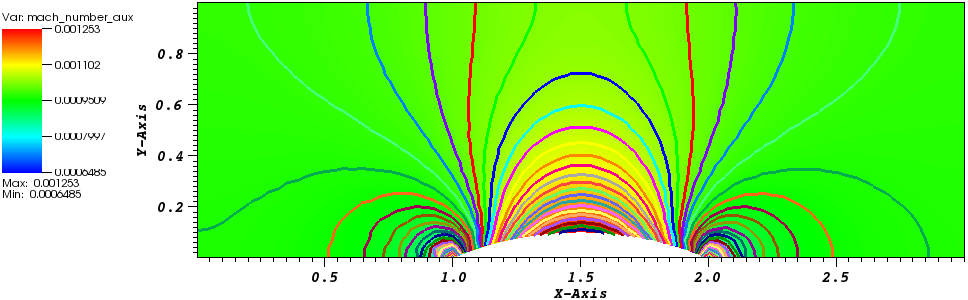
\includegraphics[height=3cm, keepaspectratio=true]{figs/Hump2D_mach_0p001.png}
  \caption{$M_{\text{inlet}}=10^{-3}$}
\end{figure}
\end{frame}

\begin{frame} 
\begin{figure}
	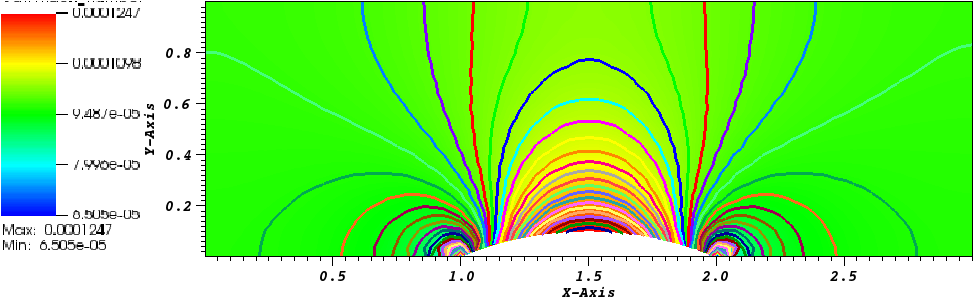
\includegraphics[height=3cm, keepaspectratio=true]{figs/Hump2D_mach_1em4.png}
  \caption{$M_{\text{inlet}}=10^{-4}$}
\end{figure}
\end{frame}

\begin{frame} 
\begin{figure}
	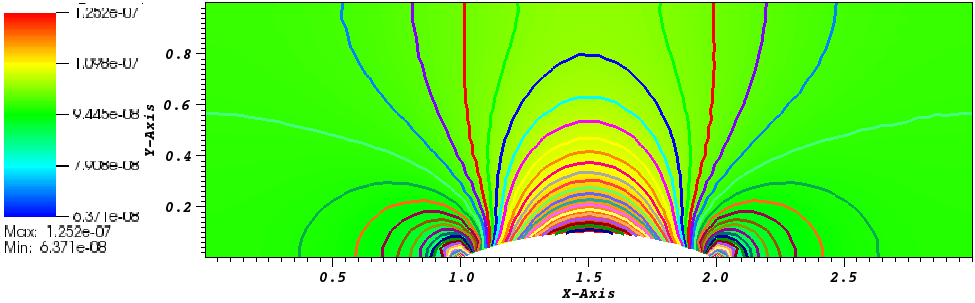
\includegraphics[height=3cm, keepaspectratio=true]{figs/Hump2D_mach_1em7.png}
  \caption{$M_{\text{inlet}}=10^{-7}$}
\end{figure}
\end{frame}

%%%%%%%%%%%%%%%%%%%%%%%%%%%%%%%%%%%%%%%%%%%%%%%%%%%%%%%%%%%%%%%%%%%%

%%%%%%%%%%%%%%%%%%%%%%%%%%%%%%%%%%%%%%%%%%%%%%%%%%%%%%%%%%%%%%%%%%%%
\begin{frame} 
\frametitle{Compression corner: Mach number contour}

\begin{center}
\movie[width=6cm,height=4cm,showcontrols=true,externalviewer]{
\includegraphics[width=6cm,height=4cm]{engr.pdf}}{movs/compression_mach_number_movie.mpeg}\\
\end{center}
\end{frame}

\begin{frame} 
\frametitle{Compression corner: viscosity contour}

\begin{center}
\movie[width=6cm,height=4cm,showcontrols=true,externalviewer]{
\includegraphics[width=6cm,height=4cm]{engr.pdf}}{movs/compression_viscosity_movie.mpeg}\\
\end{center}

\end{frame}
%%%%%%%%%%%%%%%%%%%%%%%%%%%%%%%%%%%%%%%%%%%%%%%%%%%%%%%%%%%%%%%%%%%%

%%%%%%%%%%%%%%%%%%%%%%%%%%%%%%%%%%%%%%%%%%%%%%%%%%%%%%%%%%%%%%%%%%%%
\begin{frame} 
\frametitle{Compression corner: Mach number contour}

\begin{table}[H]
\begin{center}
\begin{tabular}{|c|c|c|}  \hline
            & analytical & numerical\\ \hline
Pressure    & 2.47       & 2.467    \\ \hline
Mach number &  0.74      & 0.741    \\ \hline
Entropy     & 1.03       & 1.026    \\ \hline 
\end{tabular}
\caption{\label{tbl:corner_exact_sol} Ratio of analytical and numerical downstream to upstream quantities for 
the compression corner problems (corner angle of $15^\circ$ and inlet $M=2.5$ (analytical values from \cite{CompressionCorner}).}
\end{center}
\end{table}
%
\end{frame}
%%%%%%%%%%%%%%%%%%%%%%%%%%%%%%%%%%%%%%%%%%%%%%%%%%%%%%%%%%%%%%%%%%%%


%
%%%%%%%%%%%%%%%%%%%%%%%%%%%%%%%%%%%%%%%%%%%%%%%%%%%%%%%%%%%%%%%%%%%%%
%\section{Pressurized Nuclear Reactor (PWR) Model}
%%%%%%%%%%%%%%%%%%%%%%%%%%%%%%%%%%%%%%%%%%%%%%%%%%%%%%%%%%%%%%%%%%%%%
%
%%%%%%%%%%%%%%%%%%%%%%%%%%%%%%%%%%%%%%%%%%%%%%%%%%%%%%%%%%%%%%%%%%%%%
%\subsection{PWR Model}
%%%%%%%%%%%%%%%%%%%%%%%%%%%%%%%%%%%%%%%%%%%%%%%%%%%%%%%%%%%%%%%%%%%%%
%
%%%%%%%%%%%%%%%%%%%%%%%%%%%%%%%%%%%%%%%%%%%%%%%%%%%%%%%%%%%%%%%%%%%%%
%\begin{frame} 
%\frametitle{PWR model}
%
%Extension of the entropy viscosity method to include friction, gravity, and sink/source terms
%
%\begin{block}{Governing Laws}
%\begin{subequations}
%\begin{equation}
%\partial_t \rho + \partial_x\left( \rho u \right) = 0 
%\end{equation}
%\begin{equation}
%\partial_t \left( \rho u \right) + \partial_x\left( \rho u^2 + P \right) =  \tcb{- \frac{A}{2 D_h} \rho f |u| u - \rho g }
%\end{equation}
%\begin{equation}
%\partial_t \left( \rho E \right) + \partial_x\left[ u  \left( \rho E + P \right) \right] =\tcb{ a_w h_w \left( T - T_w \right) - \rho g u}
%\end{equation}
%\end{subequations}
%\end{block}
%
%
%We need to understand how source terms affect the entropy residual. 
%\begin{equation}
%\label{eq:equation20}
%\matder{s}= \rho \frac{s_e}{P_e}\left( \matder{P} - c^2 \matder{\rho} \right) = \frac{1}{T} \left( a_w h_w (T - T_w) + \frac{\rho}{2 D_h} f |u| u^2 \right) .
%\end{equation}
%
%We require entropy residual to grow (min. entropy principle, $\matder{s}=\partial _t s >0$). However, the sign of the wall heat source term is undetermined.\\
%
%\begin{equation}
%\label{eq:equation21}
%\mu_e(\vec{r},t) = \kappa_e(\vec{r},t) = h^2 \frac{\max\left( | \resinew(\vec{r},t) |, | R_w(\vec{r},t) | \right)}{(1-M) \rho c^2 + M \rho |\vec{u}|^2} \, \text{ with } R_w(\vec{r},t) = a_w h_w (T - T_w).
%\end{equation}
%
%\end{frame}
%%%%%%%%%%%%%%%%%%%%%%%%%%%%%%%%%%%%%%%%%%%%%%%%%%%%%%%%%%%%%%%%%%%%%
%
%
%%%%%%%%%%%%%%%%%%%%%%%%%%%%%%%%%%%%%%%%%%%%%%%%%%%%%%%%%%%%%%%%%%%%%
%\subsection{Numerical Results}
%%%%%%%%%%%%%%%%%%%%%%%%%%%%%%%%%%%%%%%%%%%%%%%%%%%%%%%%%%%%%%%%%%%%%

%%%%%%%%%%%%%%%%%%%%%%%%%%%%%%%%%%%%%%%%%%%%%%%%%%%%%%%%%%%%%%%%%%%%
%\begin{frame} 
%\frametitle{PWR model}
%
%\begin{block}{The model}
%\begin{itemize}
%%\setlength{\itemsep}{10pt}
%\item A single $1$-D channel % pipe of cross section $A=7.845 \times 10^{-5}$ $m^2$ and length $L = 3.865$ $m$.
%\item Wall friction, gravity, and wall heat source $Q_w = h_t a_w (T_{liq} - T_w)$ % with $h_t = 5.33 \times 10^4$ $W/m$, $a_w = 2.82$ $mm$.
%\item Wall temperature $T_w$ is a function of height %and computed from the model available in RELAP-7: fuel, gap and clad with a constant power $P = 7.7 \times 10^3$ $kW / m^3$.
%\item Inlet BC: specify total enthalpy ($H$) and momentum ($\rho u$).
%\item Outlet BC: static pressure boundary with $P_s = 155$ $bar$.
%\end{itemize}
%\end{block}
%
%\begin{block}{Discretization}
%\begin{itemize}
%\item Second-order accurate implicit temporal integrator (BDF2).
%\item Linear Lagrange finite elements
%\item Simulation run to steady state with a CFL of $100$.
%\end{itemize}
%\end{block}
%
%\begin{block}{Stabilization methods used}
%%The code is run with three different stabilization methods for comparison:
%\begin{itemize}
%\item entropy-viscosity method (EV).
%\item SUPG.
%\item first-order viscosity, i.e. $\mu = \mu_{max}$ (FO).
%\end{itemize}
%\end{block}
%
%
%\end{frame}
%%%%%%%%%%%%%%%%%%%%%%%%%%%%%%%%%%%%%%%%%%%%%%%%%%%%%%%%%%%%%%%%%%%%


%************************************************
%\begin{frame}{temperature and viscosity}
%\begin{figure}
    %\hspace*{-1cm}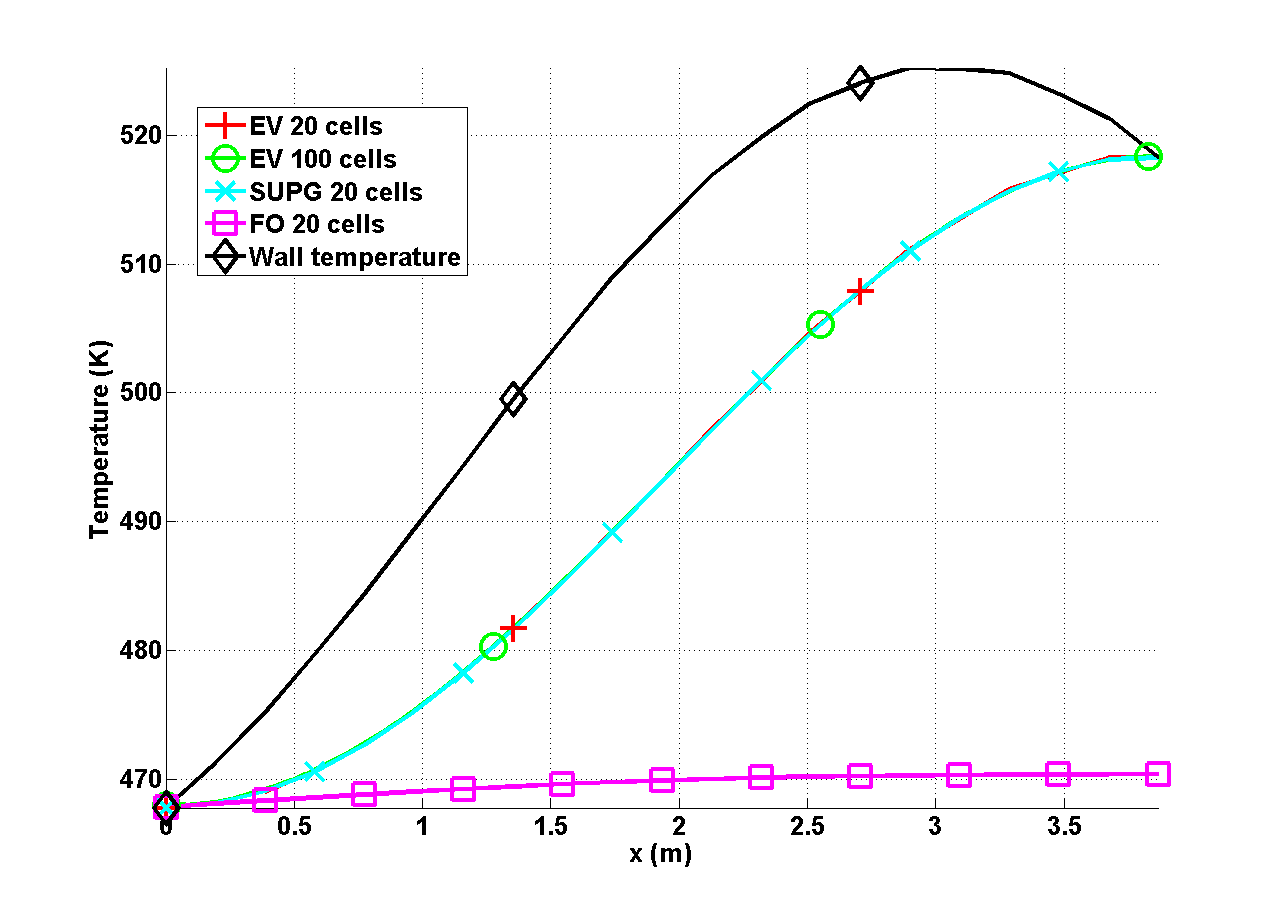
\includegraphics[width=0.65\textwidth]{figs/PWR_stt_temperature.png}
    %\hspace*{-1cm}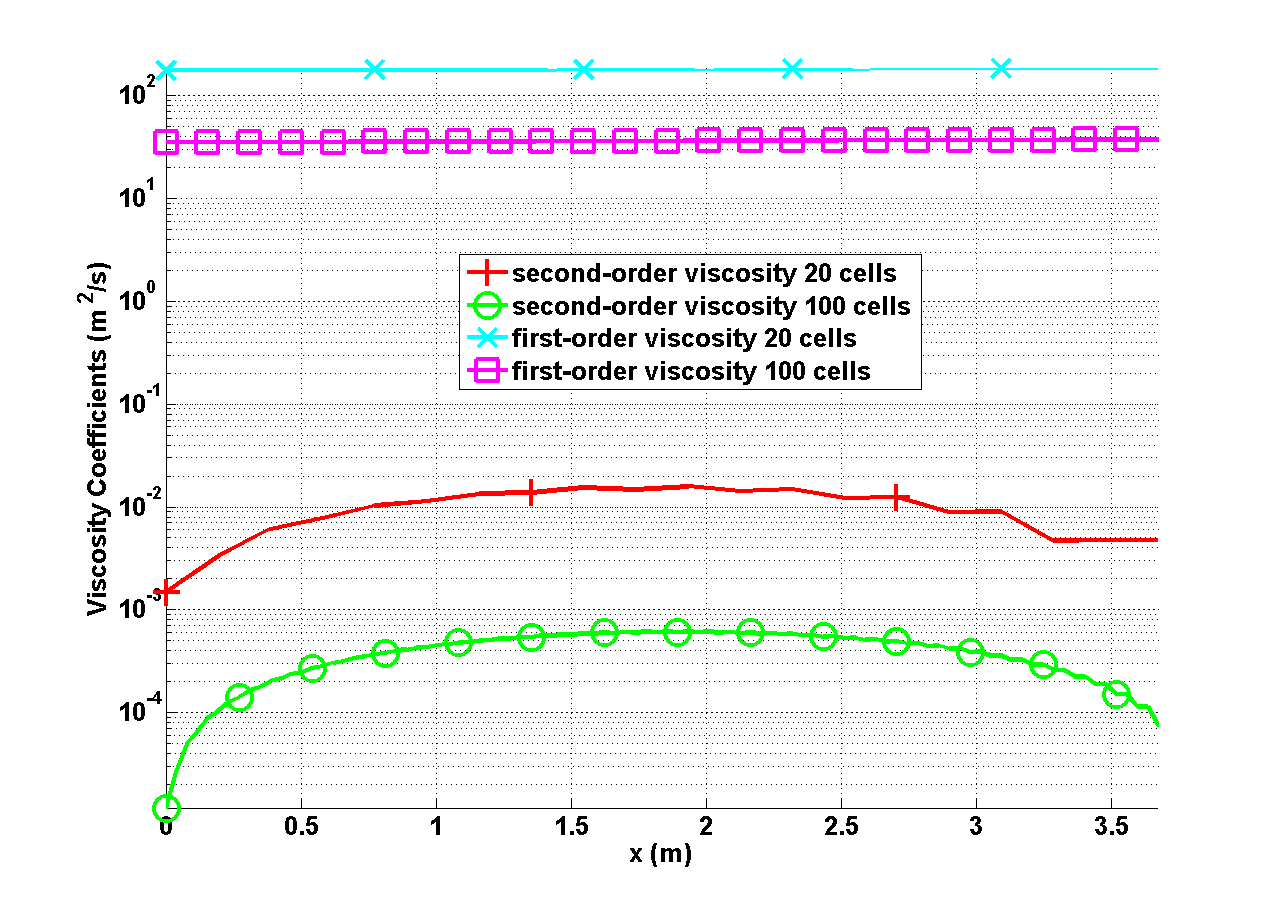
\includegraphics[width=0.65\textwidth]{figs/PWR_stt_viscosity.png}
%\end{figure}
%\end{frame}
%************************************************
%\begin{frame}{viscosity }
%\begin{figure}
    %\centering
    %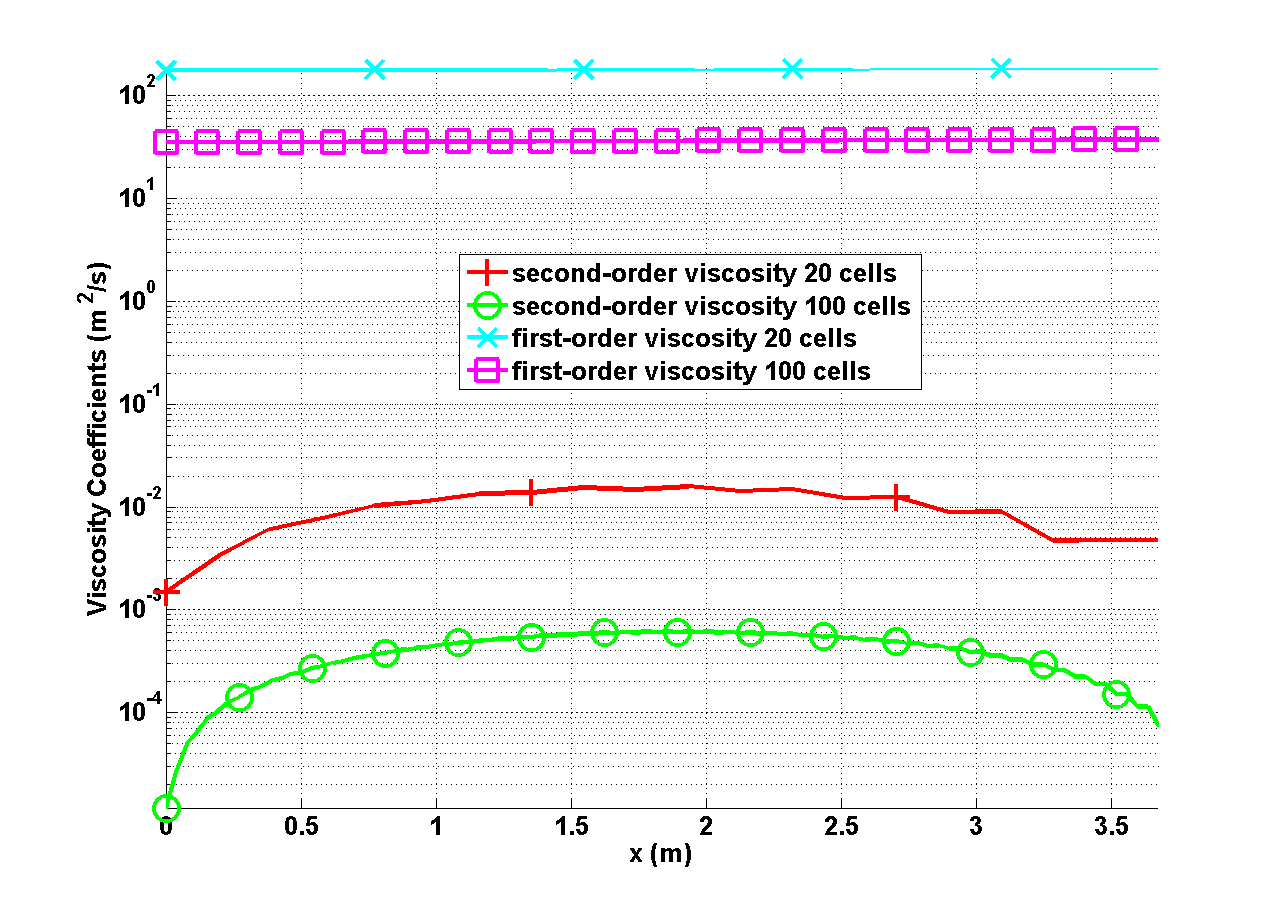
\includegraphics[width=0.98\textwidth]{figs/PWR_stt_viscosity.png}
%\end{figure}
%\end{frame}
%************************************************
%\begin{frame}{pressure and velocity}
%\begin{figure}   
    %\hspace*{-1cm}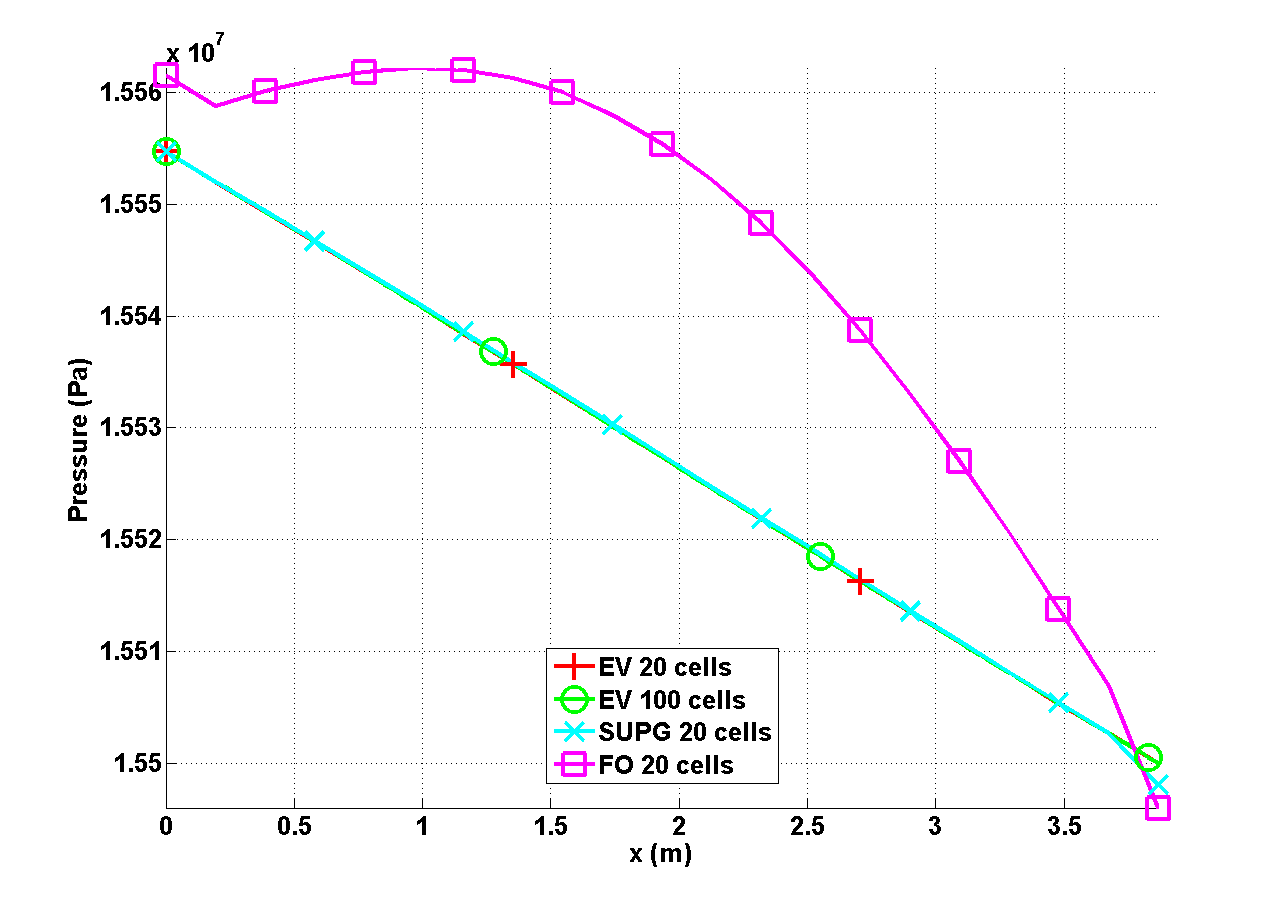
\includegraphics[width=0.65\textwidth]{figs/PWR_stt_pressure.png}
    %\hspace*{-1cm}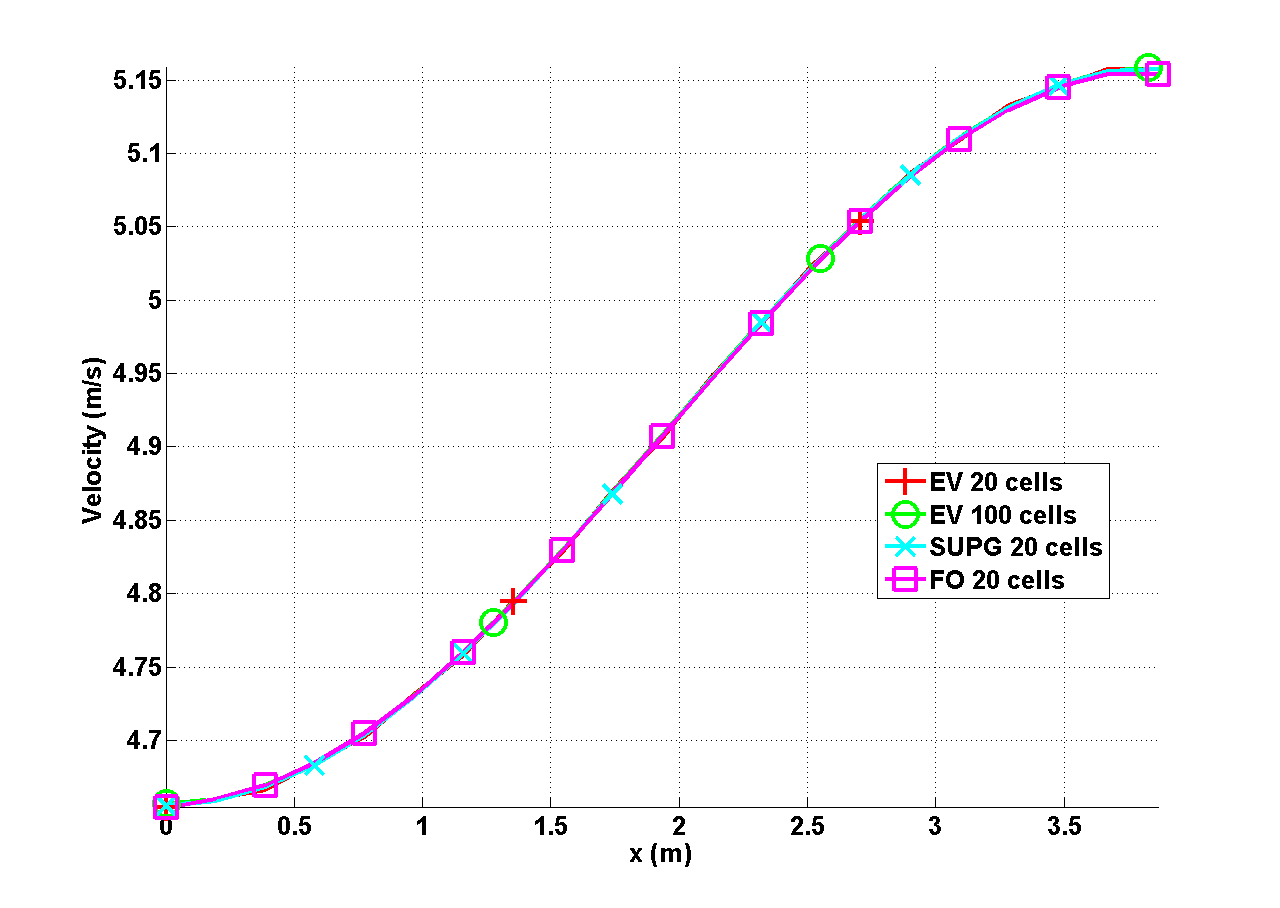
\includegraphics[width=0.65\textwidth]{figs/PWR_stt_velocity.png}
%\end{figure}
%\end{frame}
%************************************************
%\begin{frame}{velocity }
%\begin{figure}
    %\centering
    %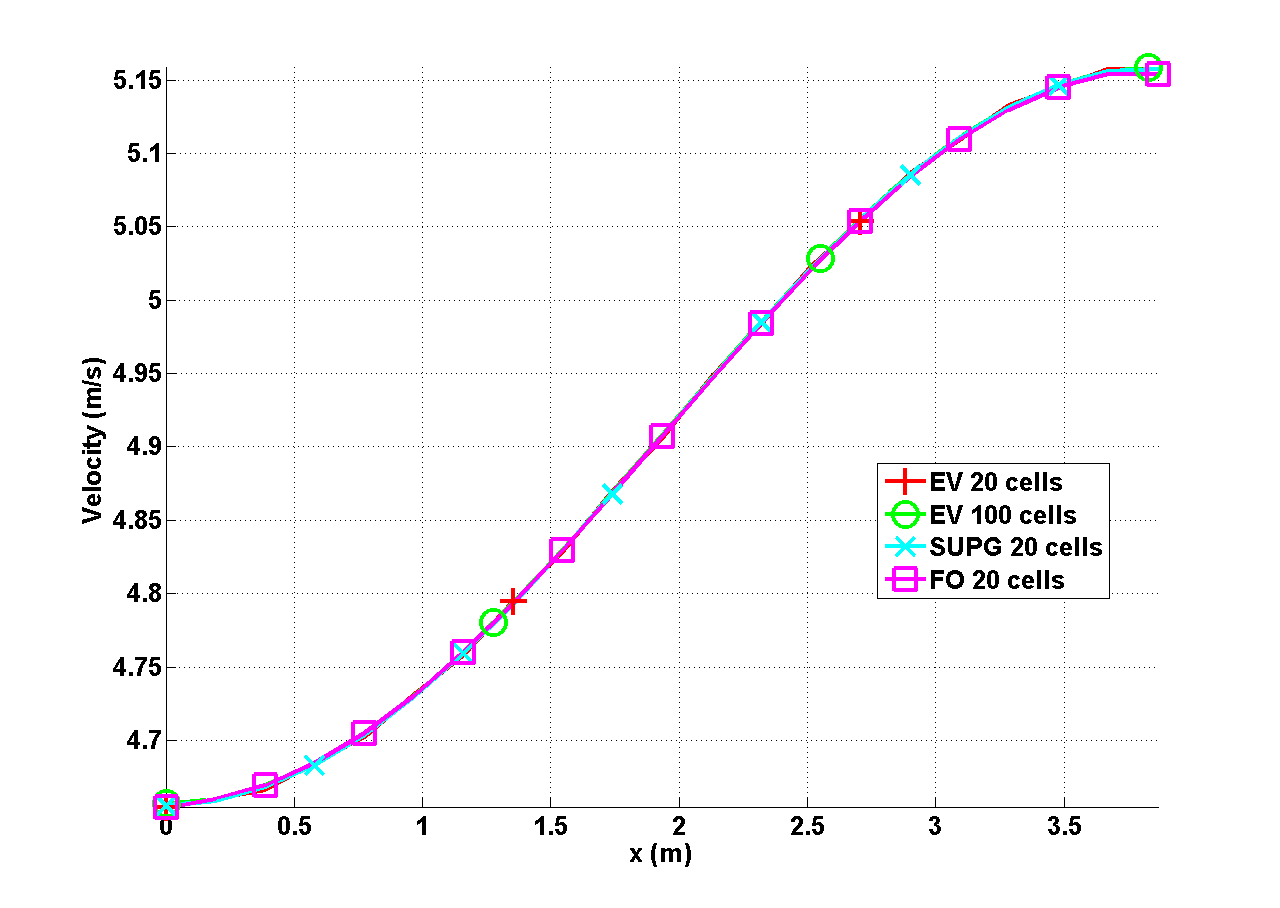
\includegraphics[width=0.98\textwidth]{figs/PWR_stt_velocity.png}
%\end{figure}
%\end{frame}
%************************************************

%\begin{frame}{PWR: mass flux steady-state profiles}
%\begin{figure}
    %\centering
    %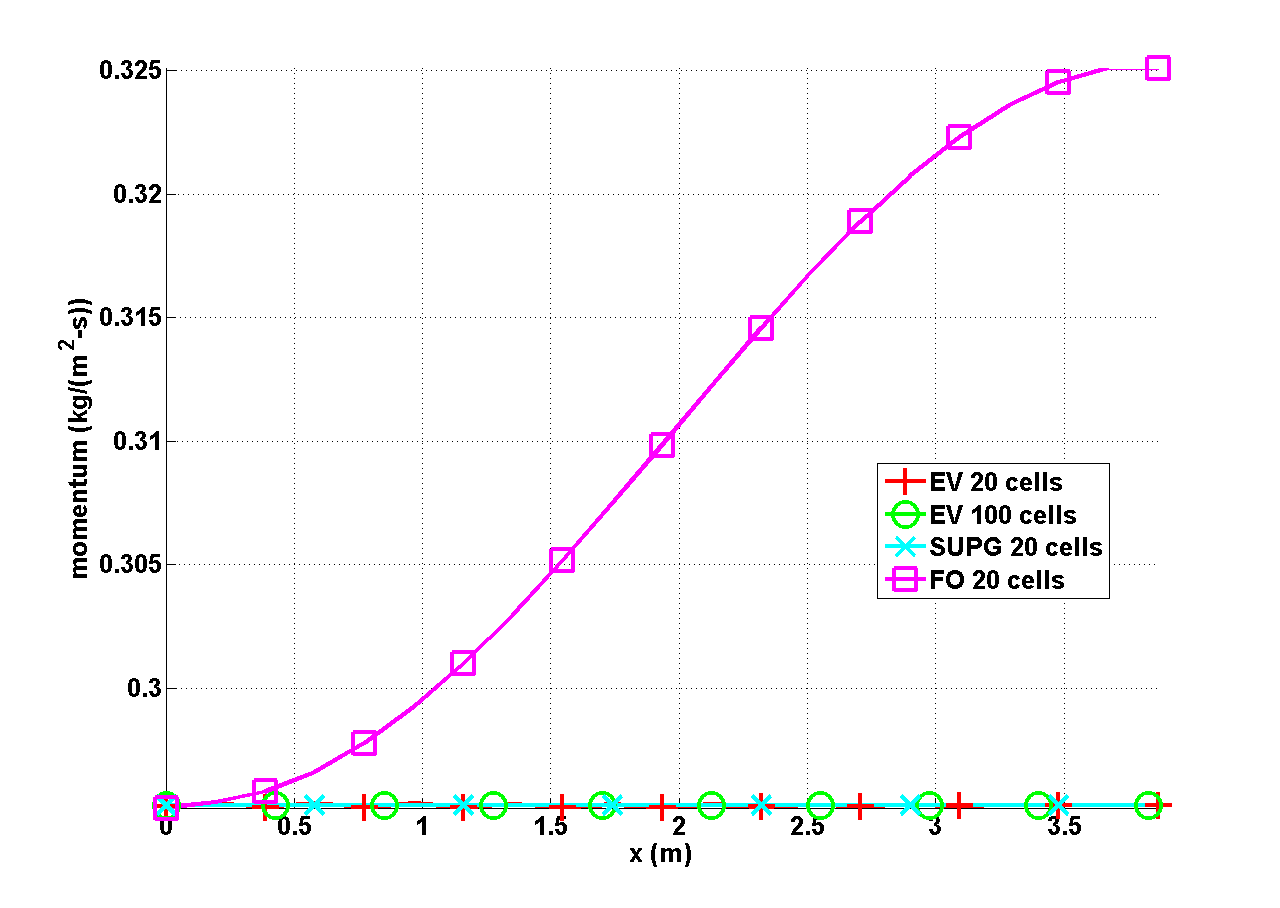
\includegraphics[width=0.98\textwidth]{figs/PWR_stt_momentum.png}
%\end{figure}
%\end{frame}
%************************************************

%%%%%%%%%%%%%%%%%%%%%%%%%%%%%%%%%%%%%%%%%%%%%%%%%%%%%%%%%%%%%%%%%%%%

%%%%%%%%%%%%%%%%%%%%%%%%%%%%%%%%%%%%%%%%%%%%%%%%%%%%%%%%%%%%%%%%%%%%
%%%%%%%%%%%%%%%%%%%%%%%%%%%%%%%%%%%%%%%%%%%%%%%%%%%%%%%%%%%%%%%%%%%%
%%%%%%%%%%%%%%%%%%%%%%%%%%%%%%%%%%%%%%%%%%%%%%%%%%%%%%%%%%%%%%%%%%%%
\section{Conclusions and Outlook}
%%%%%%%%%%%%%%%%%%%%%%%%%%%%%%%%%%%%%%%%%%%%%%%%%%%%%%%%%%%%%%%%%%%%
%%%%%%%%%%%%%%%%%%%%%%%%%%%%%%%%%%%%%%%%%%%%%%%%%%%%%%%%%%%%%%%%%%%%

%%%%%%%%%%%%%%%%%%%%%%%%%%%%%%%%%%%%%%%%%%%%%%%%%%%%%%%%%%%%%%%%%%%%
%\subsection{Conclusions}
%%%%%%%%%%%%%%%%%%%%%%%%%%%%%%%%%%%%%%%%%%%%%%%%%%%%%%%%%%%%%%%%%%%%

%%%%%%%%%%%%%%%%%%%%%%%%%%%%%%%%%%%%%%%%%%%%%%%%%%%%%%%%%%%%%%%%%%%%
\begin{frame}

\begin{block}{Conclusions}
\ben
\item Extended the entropy viscosity method to low-Mach flows
\item Presented numerical results using a \emph{continuous} FEM spatial discretization and an implicit (BDF2) temporal integration
\item Method is in RELAP-7, a MOOSE-based application of the INL
\een
\end{block}

\begin{block}{Outlook}
\ben
\item Ongoing extension the entropy viscosity method to fluid governing laws with wall heat source, wall friction, and gravity forces
\item Ongoing extension of the technique to the 7-equation two-phase flow fluid model in RELAP-7
\item Other RELAP-7 presentations: \tcb{Tuesday Nov. 11, 10:10 AM}
\een
\end{block}

\end{frame}
%%%%%%%%%%%%%%%%%%%%%%%%%%%%%%%%%%%%%%%%%%%%%%%%%%%%%%%%%%%%%%%%%%%%



%%%%%%%%%%%%%%%%%%%%%%%%%%%%%%%%%%%%%%%%%%%%%%%%%%%%%%%%%%%%%%%%%%%%
%%%%%%%%%%%%%%%%%%%%%%%%%%%%%%%%%%%%%%%%%%%%%%%%%%%%%%%%%%%%%%%%%%%%
\end{document}
